\chapter{Implementacja sprzętowa wybranych algorytmów}
\label{cha:implementacja_sprzetowa}

\section{Modele programowe}
\label{sec:modele_programowe}

\section{Wykorzystany układ oraz interfejs wizyjny}
\label{sec:uklad_interfejs}

Do implementacji algorytmów wykorzystano środowisko \textit{Vivado}. Użyto najnowszej wersji, na moment tworzenia niniejszej pracy (czerwiec 2017), oznaczonej numerem \textit{2017.1}. Większość modułów zaimplementowano w języku \textit{Verilog}. W pojedynczych przypadkach wykorzystano również język \textit{VHDL}. Wszystkie metody uruchomiono i sprawdzono na płytce \textit{VC707} z układem \textit{Virtex-7 (\small{XC7VX485T--2FFG1761})}. Jest to jeden z najwydajniejszych układów firmy \textit{Xillinx}. Dodatkowo w celu podłączenia kamery i transmisji obrazu wykorzystano kartę \textit{Avnet DVI I/O FMC}. Przyjęto założenie, że zaimplementowane algorytmy mają pracować w rozdzielczość \textit{720x576} w 50 klatkach na sekundę. Opcjonalnie obsługiwana może być również rozdzielczość \textit{1280x720} i \textit{1920x1080}, również z prędkością \textit{50 fps} (ang. \textit{Frames Per Second} -- klatki na sekundę). 
%Oprócz implementacji sprzętowych, dla każdego algorytmu przygotowano także model programowy. Modele te zostały zaimplementowane w języku \textit{C++} z wykorzystaniem biblioteki \textit{OpenCV} \cite{opencv_17}. Całość przygotowano w środowisku programistycznym \textit{Microsoft Visual Studio 2015}.

W przypadku implementacji sprzętowej w układzie \textit{FPGA} został wykorzystany uniwersalny interfejs wizyjny. Jego układ, przedstawiający podstawowe sygnały wejściowe i wyjściowe, został pokazany na rys. \ref{fig:fpga_vision_if}. Oprócz sygnałów wejściowych/wyjściowych z kamery, konieczne jest także zapewnienie niezależnego obszar pamięci \textit{RAM} dla każdego piksela. Maksymalnie do wykorzystania są 1024 bity na piksel w przypadku obrazu o rozdzielczości \textit{720x576} oraz 256 bitów dla wyższych rozdzielczości (\textit{720}p i \textit{1080}p). Sygnały pochodzące z kamery zostały szerzej opisane w rozdziale \ref{subsec:fpga_kontekst}. Należy zwrócić uwagę, że przedstawiony tutaj interfejs, zawiera jedynie niezbędne sygnały do funkcjonowania systemu. W przypadku niektórych algorytmów został on rozszerzony o dodatkowe wejścia/wyjścia. 

		\begin{figure}[h!]
				\centering
				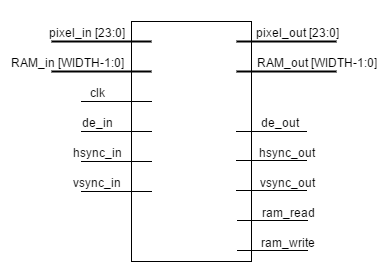
\includegraphics[scale=0.75]{img/4/vision_if.png}
				\caption{Główny interfejs wizyjny}
				\label{fig:fpga_vision_if}
		\end{figure}

\noindent \\Moduł przedstawiony na rys. \ref{fig:fpga_vision_if} posiada następujące sygnały wejściowe:\\
\-\hspace{1cm} \textit{pixel\_in} -- wartość piksela wejściowego w formacie RGB (24 bity)\\
\-\hspace{1cm} \textit{bg\_model\_in} -- odczytana pamięć RAM o długości \textit{WIDTH} (maksymalnie 1024 bity)\\
\-\hspace{1cm} \textit{clk} -- zegar piksela\\
\-\hspace{1cm} \textit{de\_in} -- flaga poprawności piksela wejściowego\\
\-\hspace{1cm} \textit{hs\_in} -- flaga synchronizacji poziomej\\
\-\hspace{1cm} \textit{vs\_in} -- flaga synchronizacji pionowej\\\\
%
Natomiast sygnałami wyjściowymi są:\\
\-\hspace{1cm} \textit{pixel\_out} -- wartość piksela wyjściowego w formacie RGB (24 bity)\\
\-\hspace{1cm} \textit{bg\_model\_out} -- blok o długości \textit{WIDTH} do zapisania w pamięci RAM (maksymalnie 1024 bity)\\
\-\hspace{1cm} \textit{de\_out} -- opóźniona flaga poprawności piksela wejściowego\\
\-\hspace{1cm} \textit{hs\_out} -- opóźniona flaga synchronizacji poziomej\\
\-\hspace{1cm} \textit{vs\_out} -- opóźniona flaga synchronizacji pionowej\\
\-\hspace{1cm} \textit{ram\_read} -- sygnał odczytu pamięci RAM\\
\-\hspace{1cm} \textit{ram\_write} -- sygnał zapisu do pamięci RAM\\

\section{Trudności występujące w potokowym systemie wizyjnym}
\label{sec:fpga_wprowadzenie}

\subsection{Kontekst poziomy i pionowy}
\label{subsec:fpga_kontekst}

Algorytmy wizyjne w układach FPGA, jak już zostało wspomniane, są realizowane w systemie potokowym. Oznacza to, że ramka obrazu przetwarzana jest piksel po pikselu. W związku z tym, w celu wykonania operacji kontekstowej koniecznej jest zastosowanie odpowiednich opóźnień. Dla kontekstu poziomego nie jest to duży problem i może zostać rozwiązany z wykorzystaniem zwykłych rejestrów. Natomiast w przypadku kontekstu pionowego konieczne jest zastosowanie opóźnienia o całą linie obrazu. Do tego celu, wykorzystuje się dostępną w układach FPGA pamięć blokową (\textit{BRAM}). Przykładowy system linii opóźniających, służących do wyznaczenia kontekstu o rozmiarze \textit{5x5} został przedstawiony na rysunku \ref{fig:fpga_delay_line}. Poprzez pojedynczy blok \textbf{D} rozumiemy opóźnienie o jeden takt zegara, z kolei stała \textit{H\_SIZE} definiuje ilość pikseli w jednej linii obrazu.

	\begin{figure}[h!]
	    \centering
		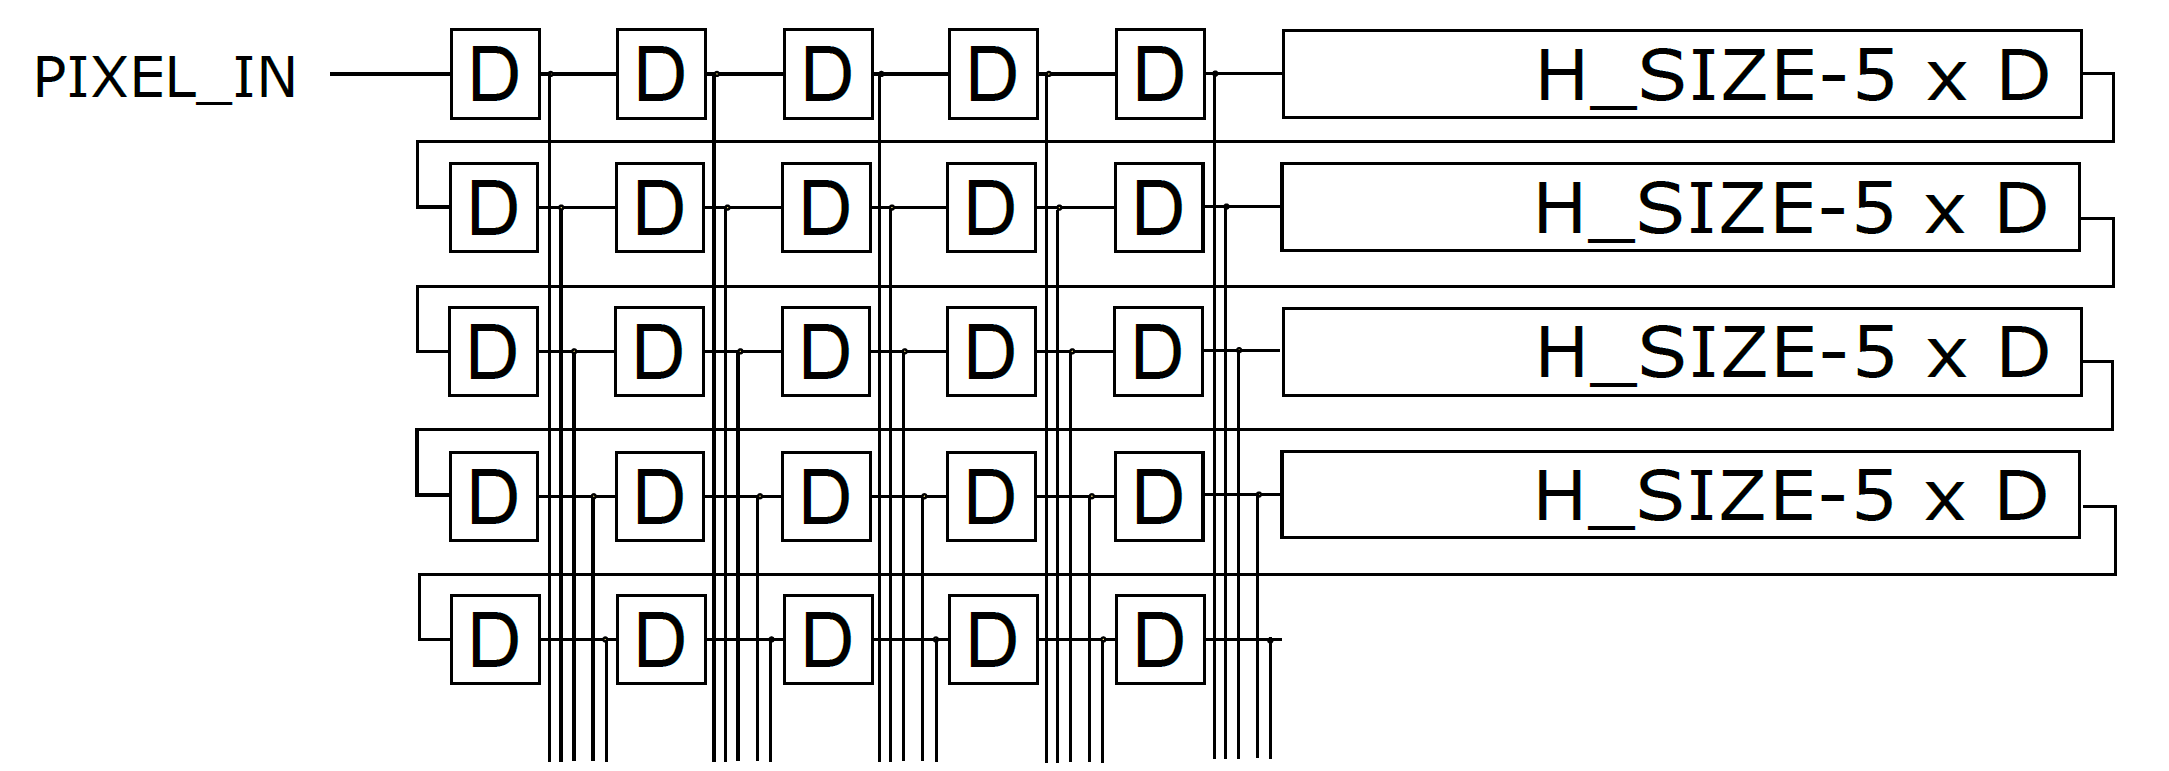
\includegraphics[scale=0.2]{img/4/context.png}
		\caption{Schemat długiej linii opóźniającej - źródło \cite{komorkiewicz_14}}
		\label{fig:fpga_delay_line}
	\end{figure}
	
Podczas ustalania parametru \textit{H\_SIZE} należy zwrócić uwagę na tzw. obszar synchronizacji. W rzeczywistość ilość pikseli przesyłanych w jednej ramce obrazu jest większa niż sugerowałaby rozdzielczość obrazu. Przykładowo, dla obrazu o rozdzielczości \textit{640x480} pikseli, rzeczywista liczba pikseli, po uwzględnieniu obszaru synchronizacji wynosi \textit{800x600}. Zostało to przedstawione na rysunku \ref{fig:fpga_sync_signals}. Wielkość obszaru synchronizacji zależy zarówno od rozdzielczości obrazu jak i liczby klatek na sekundę. Przy wyznaczaniu odpowiedniej długości, wymaganej linii opóźniającej, pomocna może okazać się baza danych \textit{Modeline Database} \cite{modeline_db_web}. W niniejszej pracy wykorzystano trzy rozdzielczości: \textit{720x576}, \textit{1280x720}, \textit{1920x1080} przy prędkości \textit{50 fps}. Całkowita długość linii poziomych, dla takich konfiguracji, wynosi odpowiednio: \textit{864}, \textit{1680}, \textit{2640}.

	\begin{figure}[h!]
        \centering
		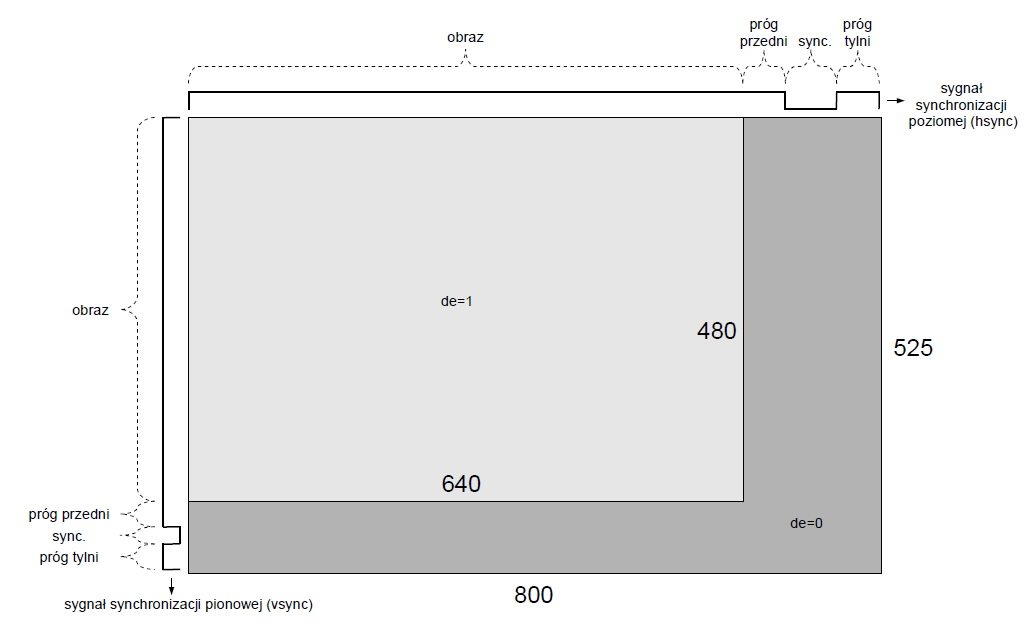
\includegraphics[scale=0.55]{img/4/sync_signals.png}
		\caption{Synchronizacja dla obrazu o rozdzielczości 640x480 -- źródło \cite{komorkiewicz_14}}
		\label{fig:fpga_sync_signals}
	\end{figure}


\subsection{Generowanie liczb losowych}
\label{subsec:fpga_generator}

Moduł odpowiedzialny za generację liczb pseudolosowych został opracowany na podstawie publikacji \cite{thomas_10}. Wykorzystano go także w wielu innych badań przeprowadzanych w Laboratorium Biocybernetyki AGH, między innymi \cite{kryjak_14_vibe, kryjak_14_pbas}. W przeciwieństwie do pozostałych modułów i algorytmów, generator został w całości zaimplementowany w języku \textit{VHDL}.

Zagadnienie liczb pseudolosowych w układach reprogramowalnych jest tematem bardzo rozległym i został dokładnie opisane w przytoczonym artykule. W niniejszym rozdziale zostanie przedstawiona jedynie skrótowa idea działania wykorzystanego generatora. Cała koncepcja opiera się na wykorzystaniu rejestrów przesuwnych (ang. \textit{shift register}) i modułów \textit{LUT} (ang. \textit{Look-Up Table}). Uproszczony schemat, tego typu generatora, zamieszczono na rysunku \ref{fig:fpga_rng}. Wartości wyjściowe są zapisywane w rejestrach przesuwnych o różnych długościach. Następnie różne kombinacje zapamiętanych bitów są podawane na wejścia bramek \textit{XOR}, które generują pseudolosowy sygnał wyjściowy.

	\begin{figure}[h!]
        \centering
		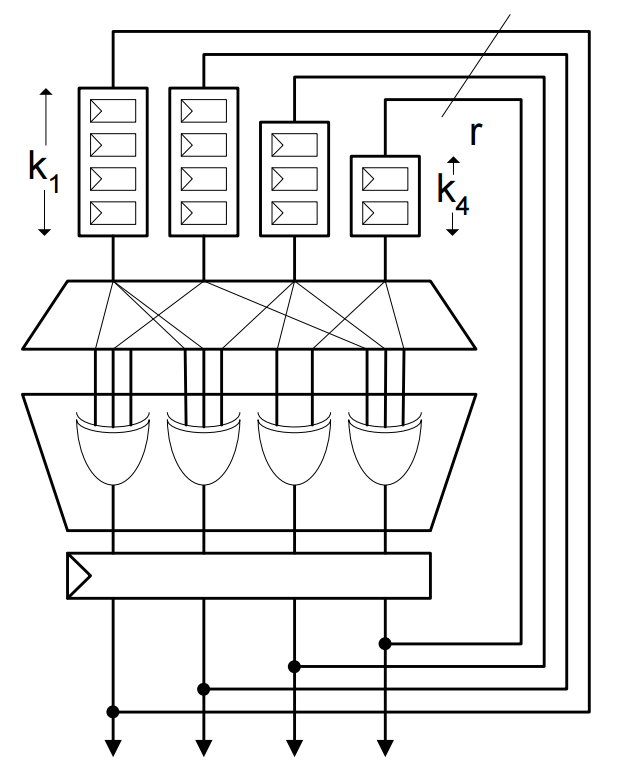
\includegraphics[scale=0.3]{img/4/rng_scheme.png}
		\caption{Schemat generatora liczb pseudolosowych -- źródło \cite{thomas_10}}
		\label{fig:fpga_rng}
	\end{figure}

Architekturę generatora można opisać za pomocą zestawu 4 parametrów ($n$, $r$, $t$, $k$), gdzie:\\
\-\hspace{1cm} \textit{n} -- liczba stanów generatora (okres możemy zapisać jako $2^n-1$)\\
\-\hspace{1cm} \textit{r} -- liczba bitów generowanych w każdym cyklu\\
\-\hspace{1cm} \textit{t} -- liczba wejść każdej bramki \textit{XOR}\\
\-\hspace{1cm} \textit{k} -- maksymalna długość rejestru przesuwnego\\

Wykorzystany w niniejszej pracy generator posiada następujące parametry: $n=3900$, $r=128$, $t=5$, $k=32$. Istnieje jeszcze jeden dodatkowy parametr $s$, który określa sposób połączeń wyjść rejestrów przesuwnych z bramkami \textit{XOR}. Dokładny algorytm, opisujący sposób doboru optymalnych połączeń, jest bardzo zaawansowanym zagadnieniem, wybiegającym poza tematykę niniejszej pracy. Szczegółowy opis i analiza tego podejścia została przedstawiona w przytoczonej publikacji.

\subsection{Kontroler pamięci RAM}
\label{subsec:fpga_ram_kontroler}

Kontroler pamięci \textit{RAM DDR3}, jest niezbędnym elementem, koniecznym do prawidłowego działa każdego rozbudowanego systemu wizyjnego. Zewnętrzna pamięć, jest bowiem niezbędna do przechowywania modelu tła dla poszczególnych pikseli. Przedstawiony kontroler, został opracowany w Laboratorium Biocybernetyki AGH w ramach publikacji \cite{kryjak_14_hd_fpga}. Podobnie jak w przypadku generatora liczb pseudolosowych, rozdział ten ma na celu jedynie przedstawienie uproszczonej koncepcji działania modułu. Dokładny opis i dyskusja zostały zawarte w przytoczonej publikacji. \textit{Xillinx} zapewnia dedykowany moduł \textit{MIG} (\textit{Memory Interface Generator}) do komunikacji z zewnętrzną pamięcią \textit{RAM}. Schemat kontrolera pamięci, wykorzystującego \textit{MIG} został przedstawiony na rysunku \ref{fig:ram_ctrl}. 

	\begin{figure}[h!]
		\centering
		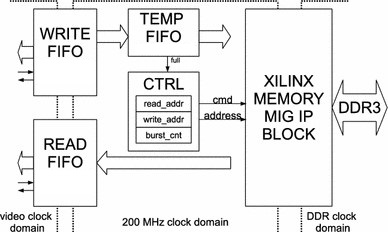
\includegraphics[scale=0.9]{img/4/ram_ctrl_scheme.jpg}
		\caption{Schemat kontrolera pamięci \textit{RAM} -- źródło \cite{kryjak_14_hd_fpga}}
		\label{fig:ram_ctrl}
	\end{figure}

Ze względu na fakt, że pamięć \textit{RAM} synchronizowana jest innym zegarem niż sygnał z kamery konieczne jest zastosowanie buforów w postaci dodatkowych kolejek \textit{FIFO}. Omawiany kontroler został zaimplementowany jako maszyna stanów. Podczas etapu inicjalizacji zapełniona zostaje w całości kolejka \textit{READ FIFO}. Następnie, w momencie gdy pojawi się na wejściu nowa ramka obrazu, modele tła z kolejki \textit{READ FIFO} zostają odczytywane i przekazywane do modułu realizującego algorytm segmentacji tła. Zaktualizowany model tła otrzymany na wyjściu, jest umieszczany w kolejce \textit{WRITE FIFO}. Kolejnym krokiem jest przeniesienie danych z kolejki \textit{WRITE FIFO} do dużo krótszej \textit{TEMP FIFO}. W~momencie, gdy kolejka ta jest zapełniona, uruchamiany jest tryb \textit{burst}, zapisujący wszystkie modele do pamięci \textit{RAM}. Po dokonaniu zapisu, dokładnie taka sama liczba modeli, zostaje odczytana z pamięci \textit{RAM} i ponownie umieszczona w kolejce \textit{READ FIFO}. Następnie kontroler przechodzi do stanu oczekiwania, aż do momentu ponownego zapełnienia się kolejki \textit{TEMP FIFO}.

\section{Implementacja algorytmu ViBE}
\label{sec:fpga_vibe}

Przygotowana implementacja sprzętowa, powstała na podstawie opisu teoretycznego metody, przedstawionego w rozdziale \ref{sec:vibe_teoria}, wykorzystano wersję operującą w przestrzeni \textit{CIELab}.  Wysokopoziomowy schemat implementacji, zawierający główny moduł realizujący algorytm, wejściowy i wyjściowy sygnał z kamery oraz połączenie z pamięcią RAM, został przedstawiony na rysunku \ref{fig:vibe_diagram}. Dla zachowania spójności, w dalszej części opisu, przyjęto oznaczenia parametrów algorytmu identyczne jak te zestawione w podsumowaniu rozdziału teoretycznego (podrozdział \ref{subsec:vibe_uwagi}).

	\begin{figure}[h!]
		\centering
		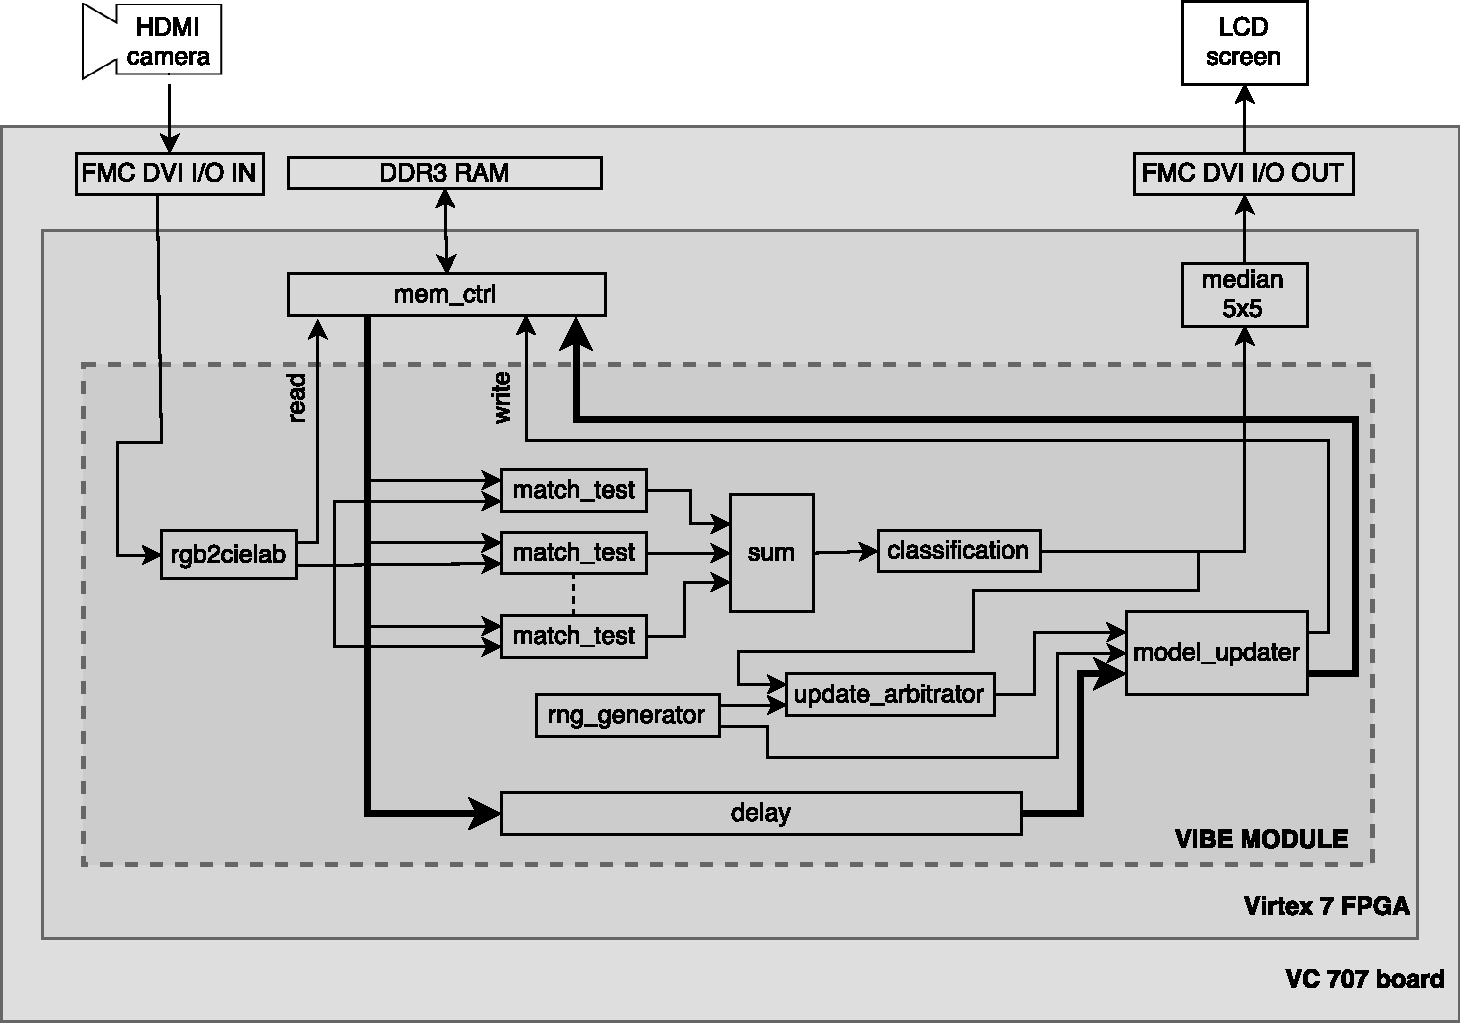
\includegraphics[scale=0.6]{img/4/vibe.pdf}
		\caption{Wysokopoziomowy schemat implementacji algorytmu \textit{ViBE}}
		\label{fig:vibe_diagram}
	\end{figure}

W podstawowej wersji algorytmu, wykorzystany został, standardowy interfejs wizyjny, przedstawiony na rysunku \ref{fig:fpga_vision_if}, bez żadnych dodatkowych sygnałów. Pierwszą operacją, jest oczywiście konwersja z przestrzeni \textit{RGB} do \textit{CIELab} (moduł \textit{rgb2cielab}). Operacja przekształcenia do macierzy \textit{XYZ}, opisana równaniem (\ref{equ:vibe_rgb_xyz}), jest prosta do zaimplementowania w logice programowej i została zrealizowana z wykorzystaniem mnożarek sprzętowych operujących na liczbach stałoprzecinkowych. Obliczanie wartości funkcji $f(t)$ zdefiniowanej równaniem (\ref{equ:vibe_f_t}) zostało zaimplementowane z użyciem operacji \textit{LUT} (ang. \textit{Look-Up Table}). Zastosowano trzy moduły, przechowujące stablicowane wartości funkcji $f(\frac{X}{X_n})$, $f(\frac{Y}{Y_n})$, $f(\frac{Z}{Z_n})$ wymagane do obliczenia składowych $a$ i $b$ danych równaniem (\ref{equ:vibe_xyz_cielab}) oraz jeden moduł zawierający wartości składowej $L$. Jak zostało już wspomniane w rozdziale \ref{subsec:vibe_cielab} składowe $a$ i $b$ mieszczą się w przedziale $-128$ do $127$. Natomiast składowa $L$ w zakresie $0$ -- $100$. W związku z tym rozmiar piksela to \textbf{23 bity} zamiast 24, jak miało to miejsce w przypadku przestrzeni \textit{RGB}.

Dla poszczególnych próbek modelu obliczany jest dystans do aktualnego piksela zgodnie z równaniem (\ref{equ:vibe_cielab_test}). Otrzymana wartość zostaje porównywana z progiem $R$. Operacje te wykonywane są równolegle dla każdej próbki z wykorzystaniem bloczków \textit{match\_test}. Następnie w module \textit{sum}, zliczane są próbki dla których test dopasowania przeszedł pozytywnie. Ostatnim etapem jest blok \textit{classification} dokonujący ostatecznej klasyfikacji piksela zgodnie z równaniem (\ref{equ:vibe_match_test}). Dodatkowo, w celu eliminacji szumów, na maskę wyjściową nakładany jest filtr medianowy o rozmiarze $5x5$.

W procesie aktualizacji modelu wykorzystywany jest, $128$ bitowy, losowy sygnał otrzymany z bloku \textit{rng\_generator}. Idea działania generatora liczb losowych została szerzej opisana w rozdziale \ref{subsec:fpga_generator}. Modułu \textit{update\_arbitrator} jest wykorzystywany do podejmowania decyzji odnośnie aktualizacji. Sama aktualizacja wykonywana jest natomiast w bloku \textit{model\_updater}. W tym celu, generowany jest kontekst o rozmiarze $3x3$, zawierający modele tła sąsiadujących pikseli. Na podstawie informacji, otrzymanych z modułu \textit{update\_arbitrator}, aktualizowany jest model piksela oraz losowo wybranego sąsiada. Następnie nowy model zostaje zapisany do pamięci \textit{RAM}. Warto zwrócić uwagę, że model jest odczytywany z pamięci po konwersji do przestrzeni \textit{CIELab}, aby wykorzystać go w procesie aktualizacji, konieczne jest zastosowanie linii opóźniającej o długości równej latencji procesu klasyfikacji piksela, operacja ta została zrealizowana przez moduł \textit{delay}.

Przedstawioną implementację udało się uruchomić w rozdzielczościach: \textit{576p}, \textit{720p}, \textit{1080p}. Na rysunku \ref{fig:vibe_demo} przedstawiono zdjęcie działającego systemu. W przypadku najniższej rozdzielczości przyjęto model składający się z $N=20$ próbek (rozmiar modelu wynosi w tym przypadku $20 \cdot 23=460$ bitów). Dla wyższych rozdzielczości, ze względu na ograniczenia pamięci \textit{RAM}, musiał on zostać ograniczony do $10$ (rozmiar modelu równy $10 \cdot 23=230$ bity). Pozostałym parametrom przypisano wartości domyślne, zostały one zapisane jako liczny całkowite. Wyjątkiem jest parametr $T$, opisujący prawdopodobieństwo wykonania aktualizacji, w tym przypadku została wykorzystana 16 bitowa liczba stałoprzecinkowa (ang. \textit{fixed float}) bez znaku o oznaczeniu \textit{8z8u}, czyli po 8 bitów przeznaczonych na część całkowitą i ułamkową.

	\begin{figure}[h!]
		\centering
		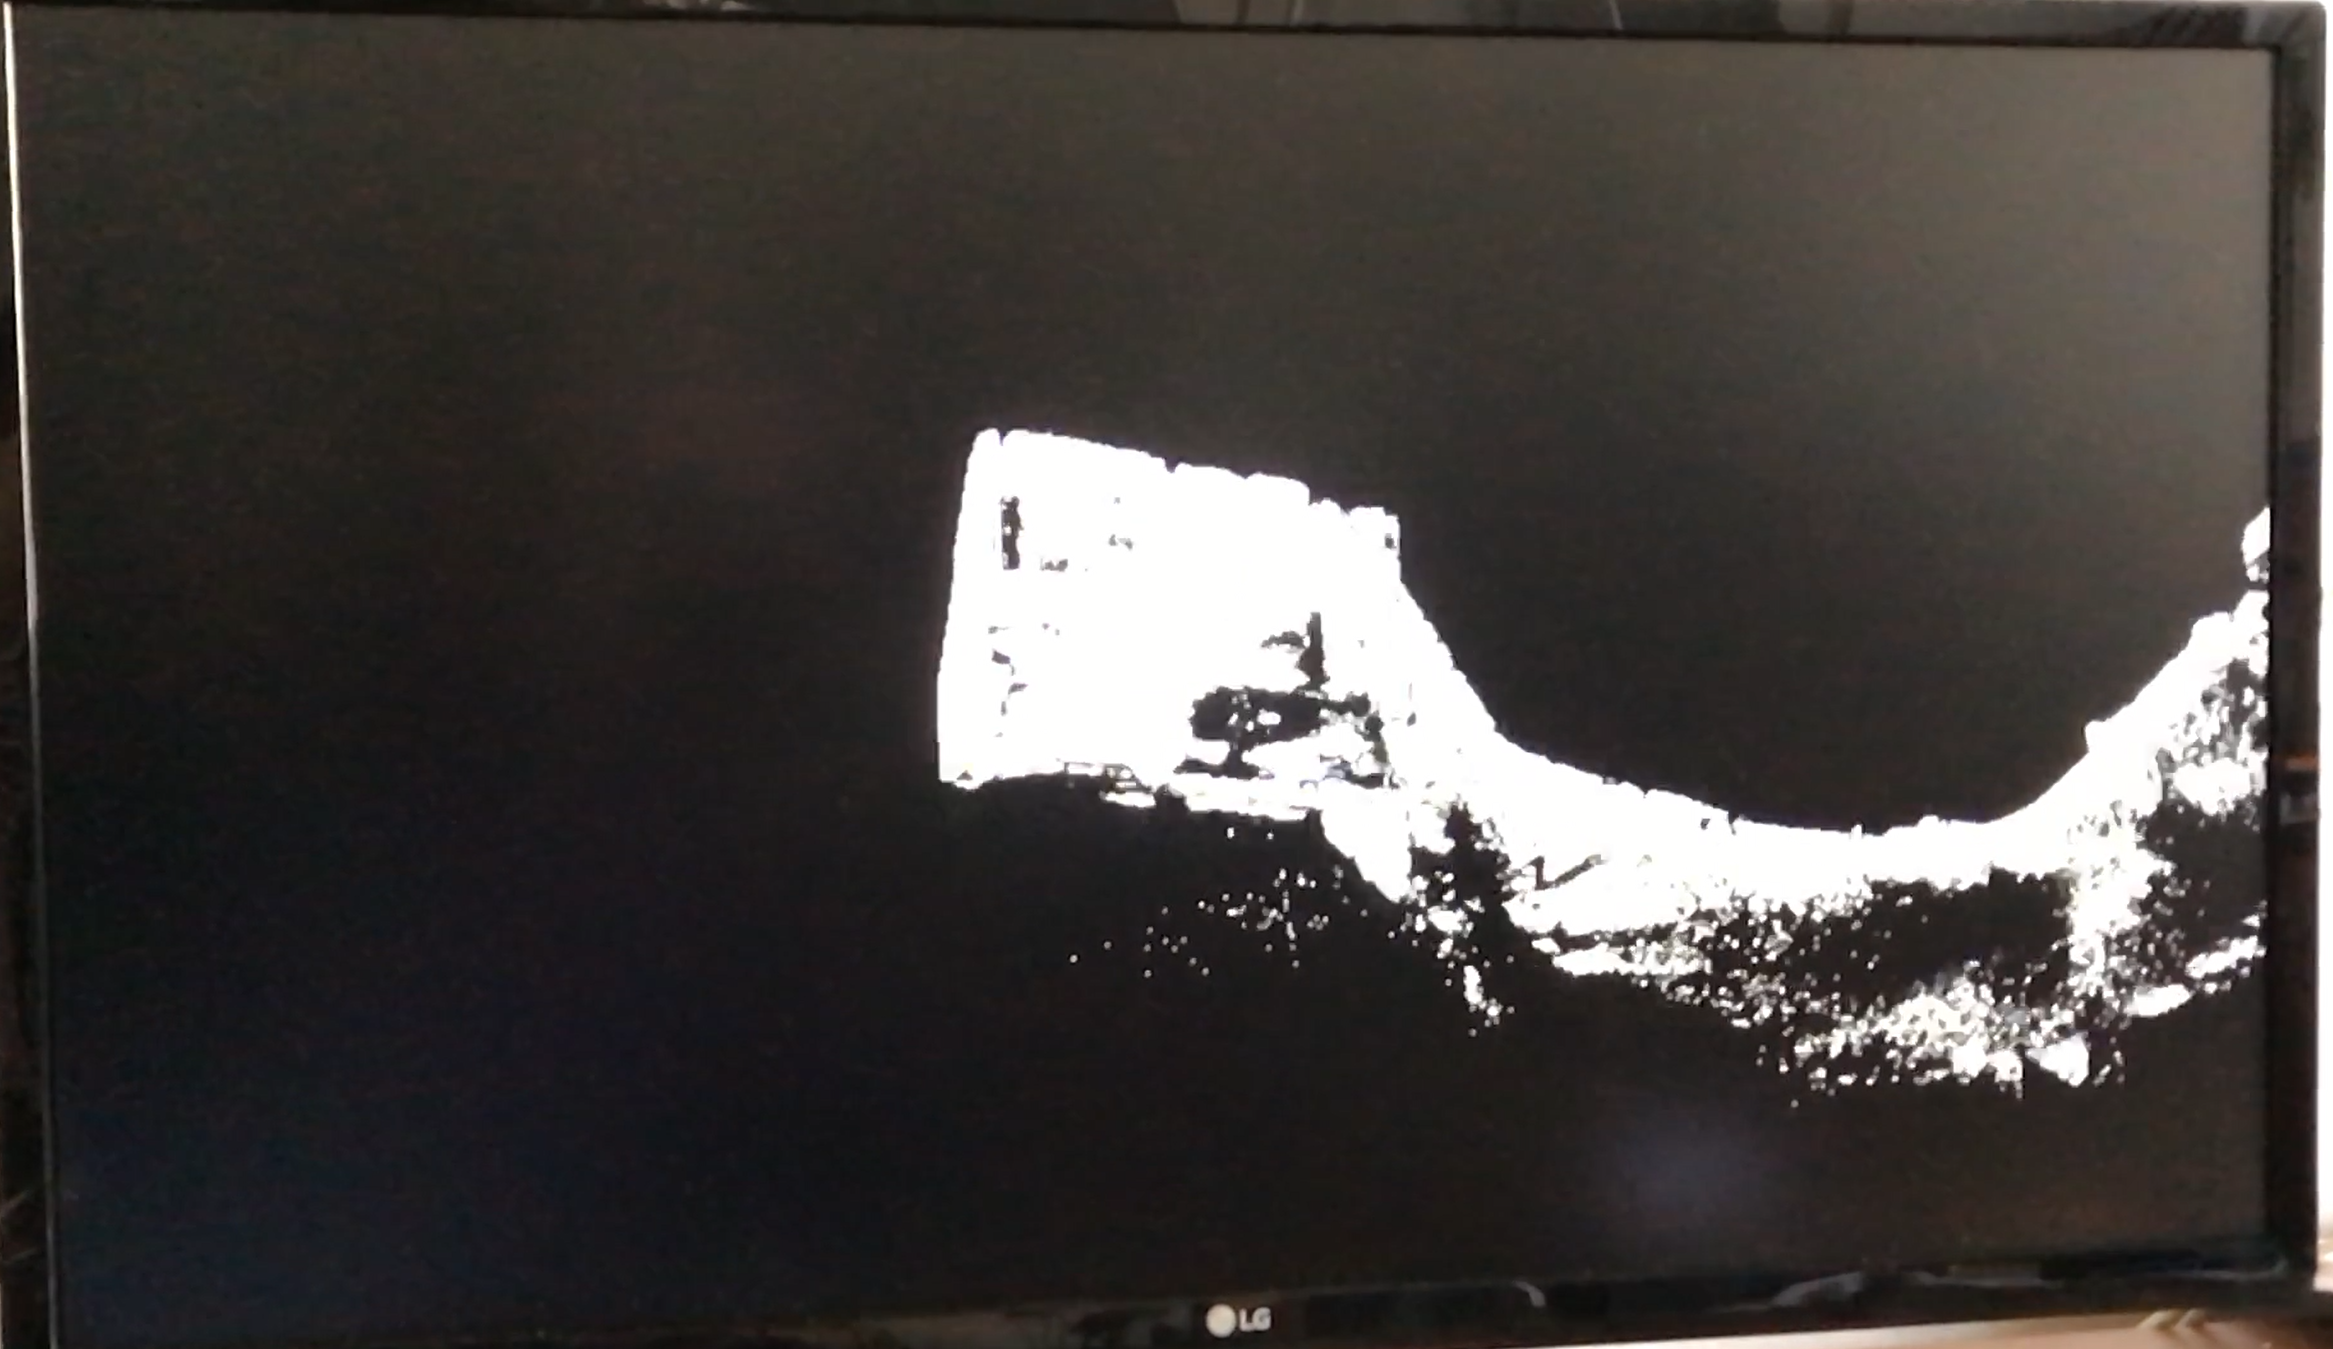
\includegraphics[scale=0.2]{img/4/vibe_example.png}
		\caption{Działający algorytm \textit{ViBE}}
		\label{fig:vibe_demo}
	\end{figure}	
	
	
\section{Implementacja rozszerzonej wersji ViBE}
\label{sec:fpga_vibe_plus}

W rozdziale \ref{subsec:vibe_ruchoma_kamera} opisany został dodatkowy mechanizm, usprawniający pracę algorytmu w przypadku występowania drgań kamery (ang. \textit{camera jitter}). Schemat implementacji rozszerzonej wersji algorytmu, zawierającej ten dodatkowy moduł, został przedstawiony na rysunku \ref{fig:vibe_plus_diagram}. Implementacja odpowiada opisowi teoretycznemu, który został przedstawiony w podrozdziale \ref{subsec:vibe_ruchoma_kamera}. Oprócz bloku realizującego standardowy algorytm \textit{ViBE}, opisanego szczegółowo w poprzednim rozdziale, ta wersja algorytmu zawiera także szereg modułów zapewniających prawidłowe przesunięcie modelu tła na podstawie wyznaczonego przepływu optycznego. Moduł, podobnie jak poprzednia wersja, wykorzystuje standardowy interfejs wizyjny, schemat modelu tła jest również identyczna jak w podstawowej wersji algorytmu. 
	
	\begin{figure}[h!]
		\centering
		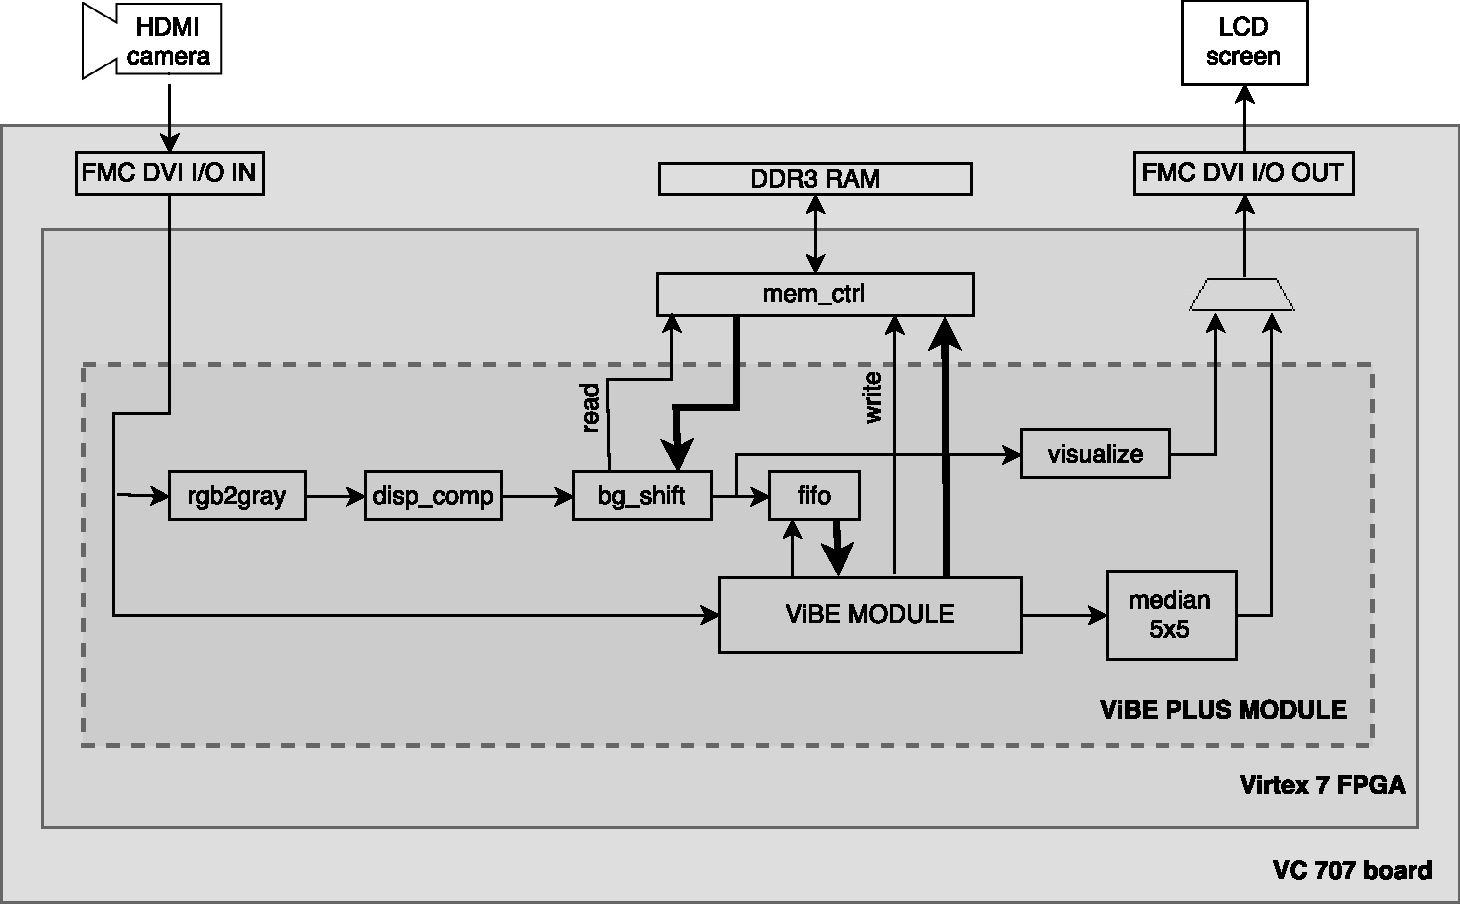
\includegraphics[scale=0.6]{img/4/vibe_plus.pdf}
		\caption{Wysokopoziomowy schemat implementacji rozszerzonego algorytmu \textit{ViBE}}
		\label{fig:vibe_plus_diagram}
	\end{figure}

Pierwszym krokiem, podczas obliczania przepływu optycznego, jest konwersja obrazu z przestrzeni \textit{RGB} do skali szarości. Jest to wykonywane poprzez moduł \textit{rgb2gray}. Przekształcony sygnał z kamery jest następnie podawany na wejście bloku \textit{disp\_comp}, realizującego operację wyznaczania przesunięcia modelu na podstawie wyliczonego przepływu optycznego. Jest to najbardziej złożony moduł w całej implementacji. Jego szczegółowy schemat został przedstawiony na rysunku \ref{fig:displacement_diagram}. Na podstawie otrzymanego wektora przesunięcia blok \textit{bg\_shift} zapewnia prawidłową synchronizację i odczyt kolejnych modeli tła z~pamięci \textit{RAM}. Ze względu na przesunięcie, operacja odczytu, musi zostać wykonana z odpowiednim wyprzedzeniem lub opóźnieniem. Dane z pamięci \textit{RAM} są umieszczane w kolejce \textit{FIFO} (ang. \textit{First In First Out} -- pierwszy na wejściu, pierwszy na wyjściu). Skąd następnie są pobierane przez algorytm \textit{ViBE}. Kolejka \textit{FIFO}, podobnie jak linie opóźniające, została zaimplementowana z wykorzystaniem pamięci blokowej (\textit{BRAM}). Dzięki zastosowaniu uniwersalnego interfejsu z niezależnymi sygnałami odczytu i~zapisu do pamięci RAM, nie było konieczności modyfikowania oryginalnej implementacji metody \textit{ViBE}. Na maskę wyjściową, nakładany jest filtr medianowy o rozmiarze $5x5$, dodatkowo został zaimplementowany moduł wizualizujący operację obliczania przepływu optycznego.

Rozszerzona wersja algorytmu operuje jedynie na rozdzielczości \textit{720x576}. Zastosowano identyczne parametry jak w podstawowej wersji metody, czyli model tła składający się z 20 próbek w przestrzeni \textit{CIELab}. Składowa wektora przesunięcia może przyjąć maksymalnie wartość $32$, zatem kolejka \textit{FIFO} gromadząca modele tła musi mieć długość $32 \cdot$\textit{H\_SIZE}$+32$, gdzie każdy element ma szerokość równą modelowi tła. Dla obsługiwanej rozdzielczości parametr \textit{H\_SIZE} wynosi 864, natomiast model tła ma rozmiar 460 bitów. Ostatecznie ustawiono szerokość pojedynczego elementu na 512 bitów, natomiast głębokość kolejki wynosi 32768.  

	\begin{figure}[h!]
		\centering
		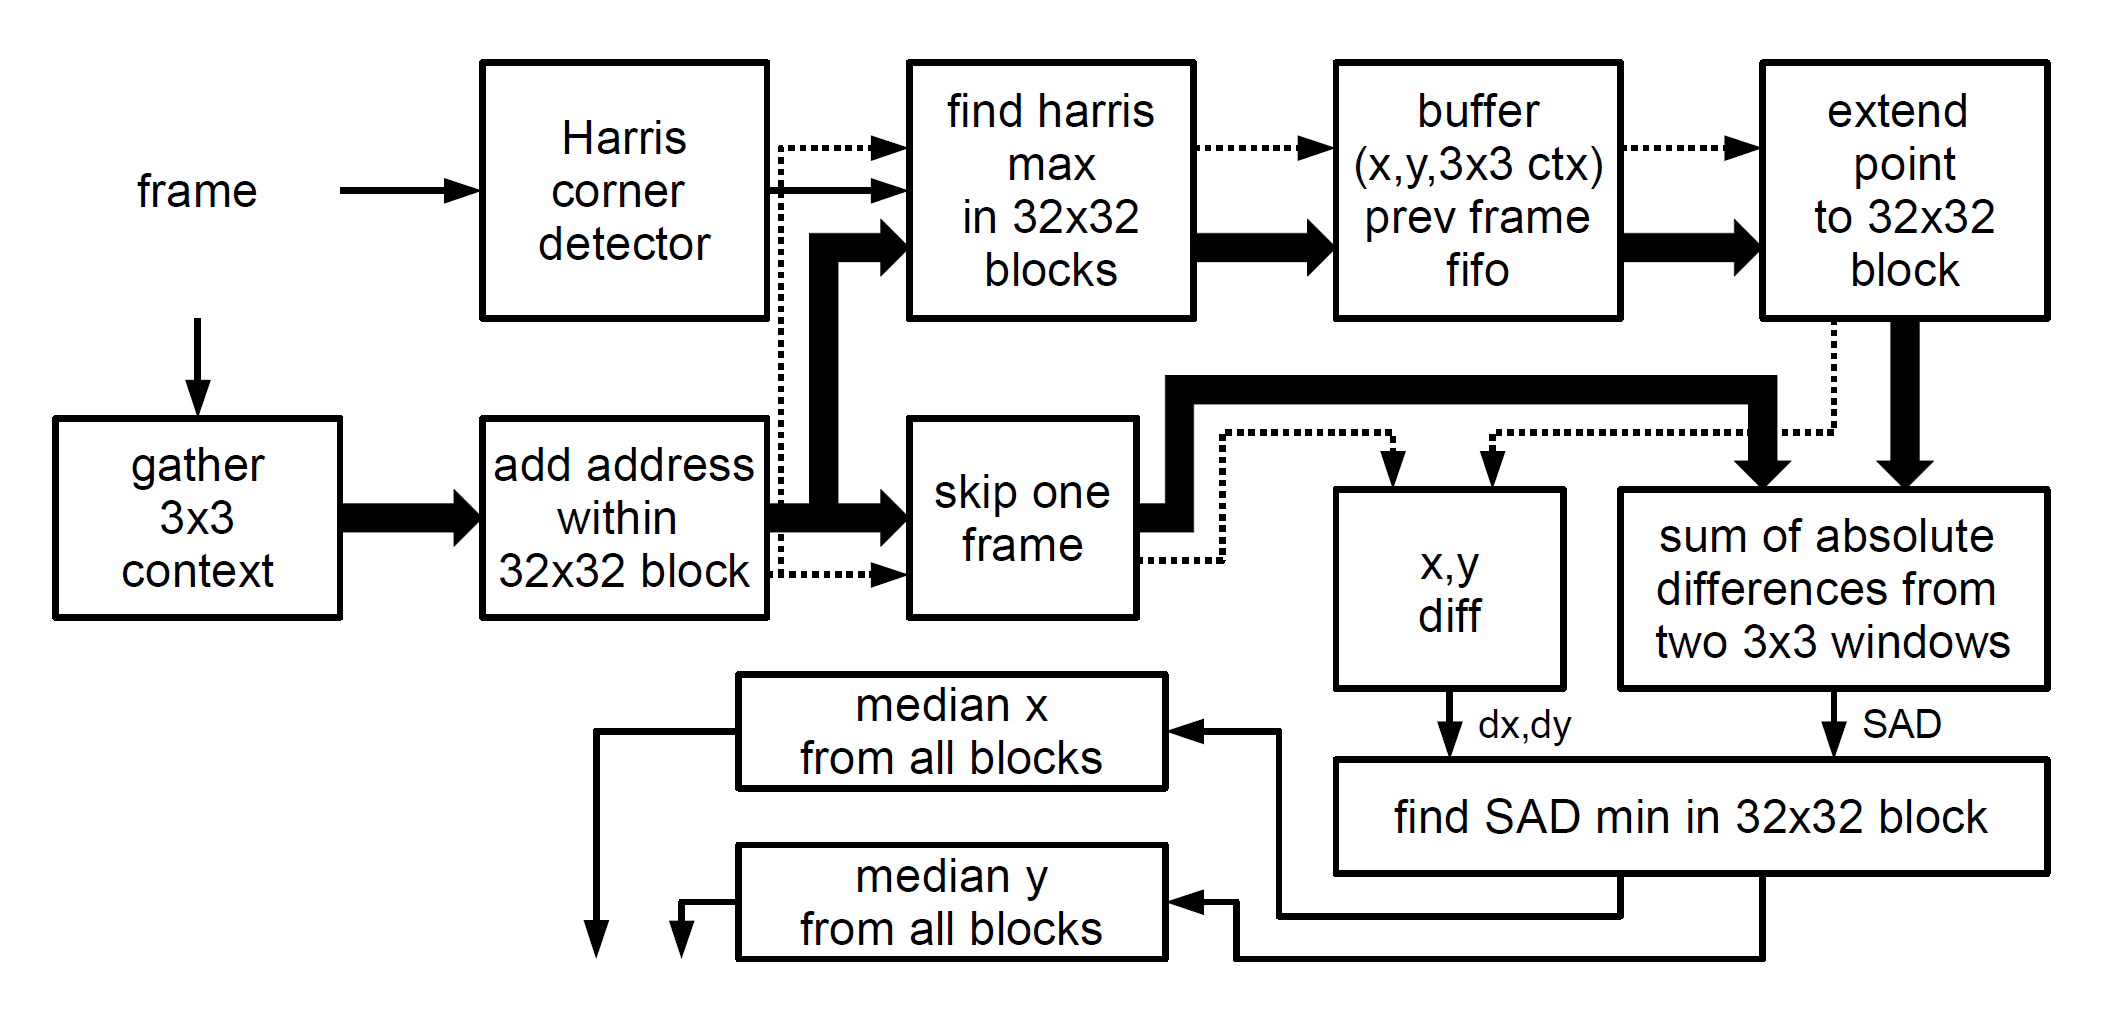
\includegraphics[scale=0.25]{img/4/displacement_vector_diagram.png}
		\caption{Implementacja modułu wyznaczającego wektor przesunięcia -- źródło \cite{}}
		\label{fig:displacement_diagram}
	\end{figure}

Moduł realizujący wyznaczanie wektora przesunięcia, jest najbardziej złożonym elementem algorytmu. Opis teoretyczny tej metody został przedstawiony w podrozdziale \ref{subsec:vibe_of}. pierwszym krokiem algorytmu jest detekcja narożników metodą Harrisa-Stephensa. Schemat przedstawiający implementację tej funkcji został pokazany na rysunku \ref{fig:harris_diagram}. Wykonane tam operacje odpowiadają opisowi teoretycznemu zamieszczonemu w podrozdziale \ref{subsec:vibe_harris}. Przy implementacji uwzględniono w maksymalnym stopniu możliwości układu FPGA w zakresie zrównoleglania obliczeń. Moduły \textit{prewitt\_x} i \textit{prewitt\_y} realizują detekcję krawędzi pionowych i poziomych. Następnie wszystkie trzy elementy macierzy $H$ są obliczane równolegle. Po dokonaniu operacji wygładzania filtrem Gaussa (blok \textit{gaussian\_blur}) w bloku \textit{rescaling} następuje przeskalowanie (dzielenie przez $2^10$) otrzymanych wartości. Finalnie wyznaczany jest wyznacznik macierzy $H$, zgodnie z równaniem (\ref{equ:vibe_harris_response_final}). Całość została zrealizowana z wykorzystaniem sprzętowych mnożarek i sumatorów. Konieczne jest wykonanie 6 operacji mnożenia, jednego dodawania i dwóch odejmowania.
 
	\begin{figure}[h!]
		\centering
		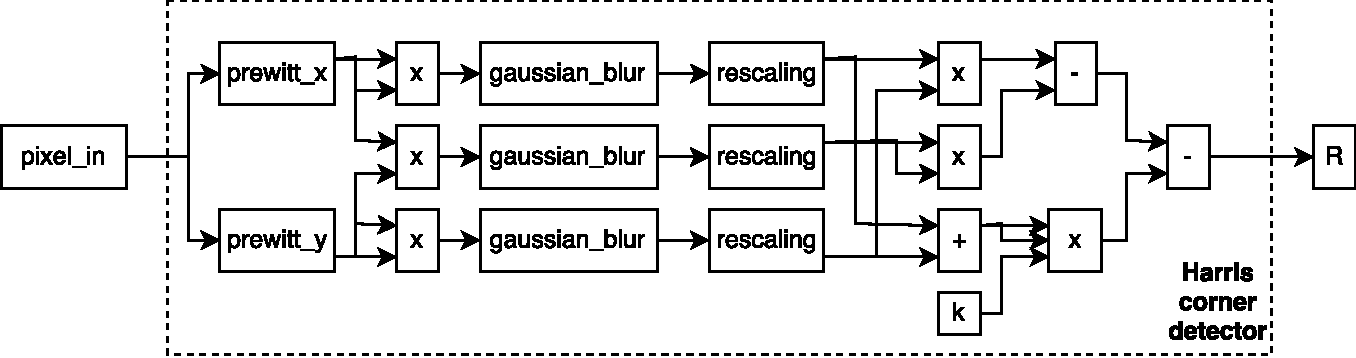
\includegraphics[scale=0.6]{img/4/harris_detector.pdf}
		\caption{Moduł realizujący detekcję narożników metodą Harrisa-Stephensa}
		\label{fig:harris_diagram}
	\end{figure}

Równolegle do detekcji krawędzi wyznaczany jest kontekst aktualnego piksela o rozmiarze $3x3$, określana jest także jego pozycja w aktualnie przetwarzanym bloku o rozmiarze $32x32$. Piksel dla którego otrzymano najmniejszą wartość współczynnika $R$ w obszarze każdego bloku zostaje zapisany razem z kontekstem $3x3$ w kolejce \textit{FIFO} (w przypadku obrazu o rozdzielczości \textit{720x576} konieczne jest zdefiniowanie kolejki o rozmiarze 396, gdyż tyle jest bloków $32x32$ w jednej ramce). Kolejne elementy z~kolejki, są pobierane w trakcie przetwarzania następnej ramki obrazu. W każdym z bloków znajdowana jest minimalna wartość sumy różnicy modułów pomiędzy pikselem pobranym z kolejki i pikselami z~aktualnej ramki obrazu. Znaleziona wartość, wraz z wektorem przesunięcia, zostaje po raz kolejny zapamiętana w pamięci blokowej. 

Ostatnim krokiem, jest obliczenie mediany przesunięcia $dx$ i $dy$ wśród znalezionych wartości minimalnych. Operacja ta, składa się z dwóch etapów, wykonywanych w momencie przerwy pomiędzy kolejnymi ramkami obrazu (wartość sygnału \textit{vsync} wynosi wtedy $0$). Najpierw wyliczany jest histogram wartości $dx$ i $dy$, równolegle zliczana jest także ilość próbek. Drugim krokiem jest sumowanie wartości histogramu. Poprzez mediane, rozumiemy wartość, dla której aktualna suma wartości histogramu jest większa niż połowa liczby wszystkich próbek. Do obliczenia histogramu ponownie został wykorzystany moduł pamięci blokowej (\textit{BRAM}). Na rysunku \ref{fig:vibe_plus_demo} przedstawiono wizualizację wyznaczanego przepływu optycznego, analogiczną do tej pokazanej na rysunku \ref{fig:vibe_of_example}.

	\begin{figure}[h!]
		\centering
		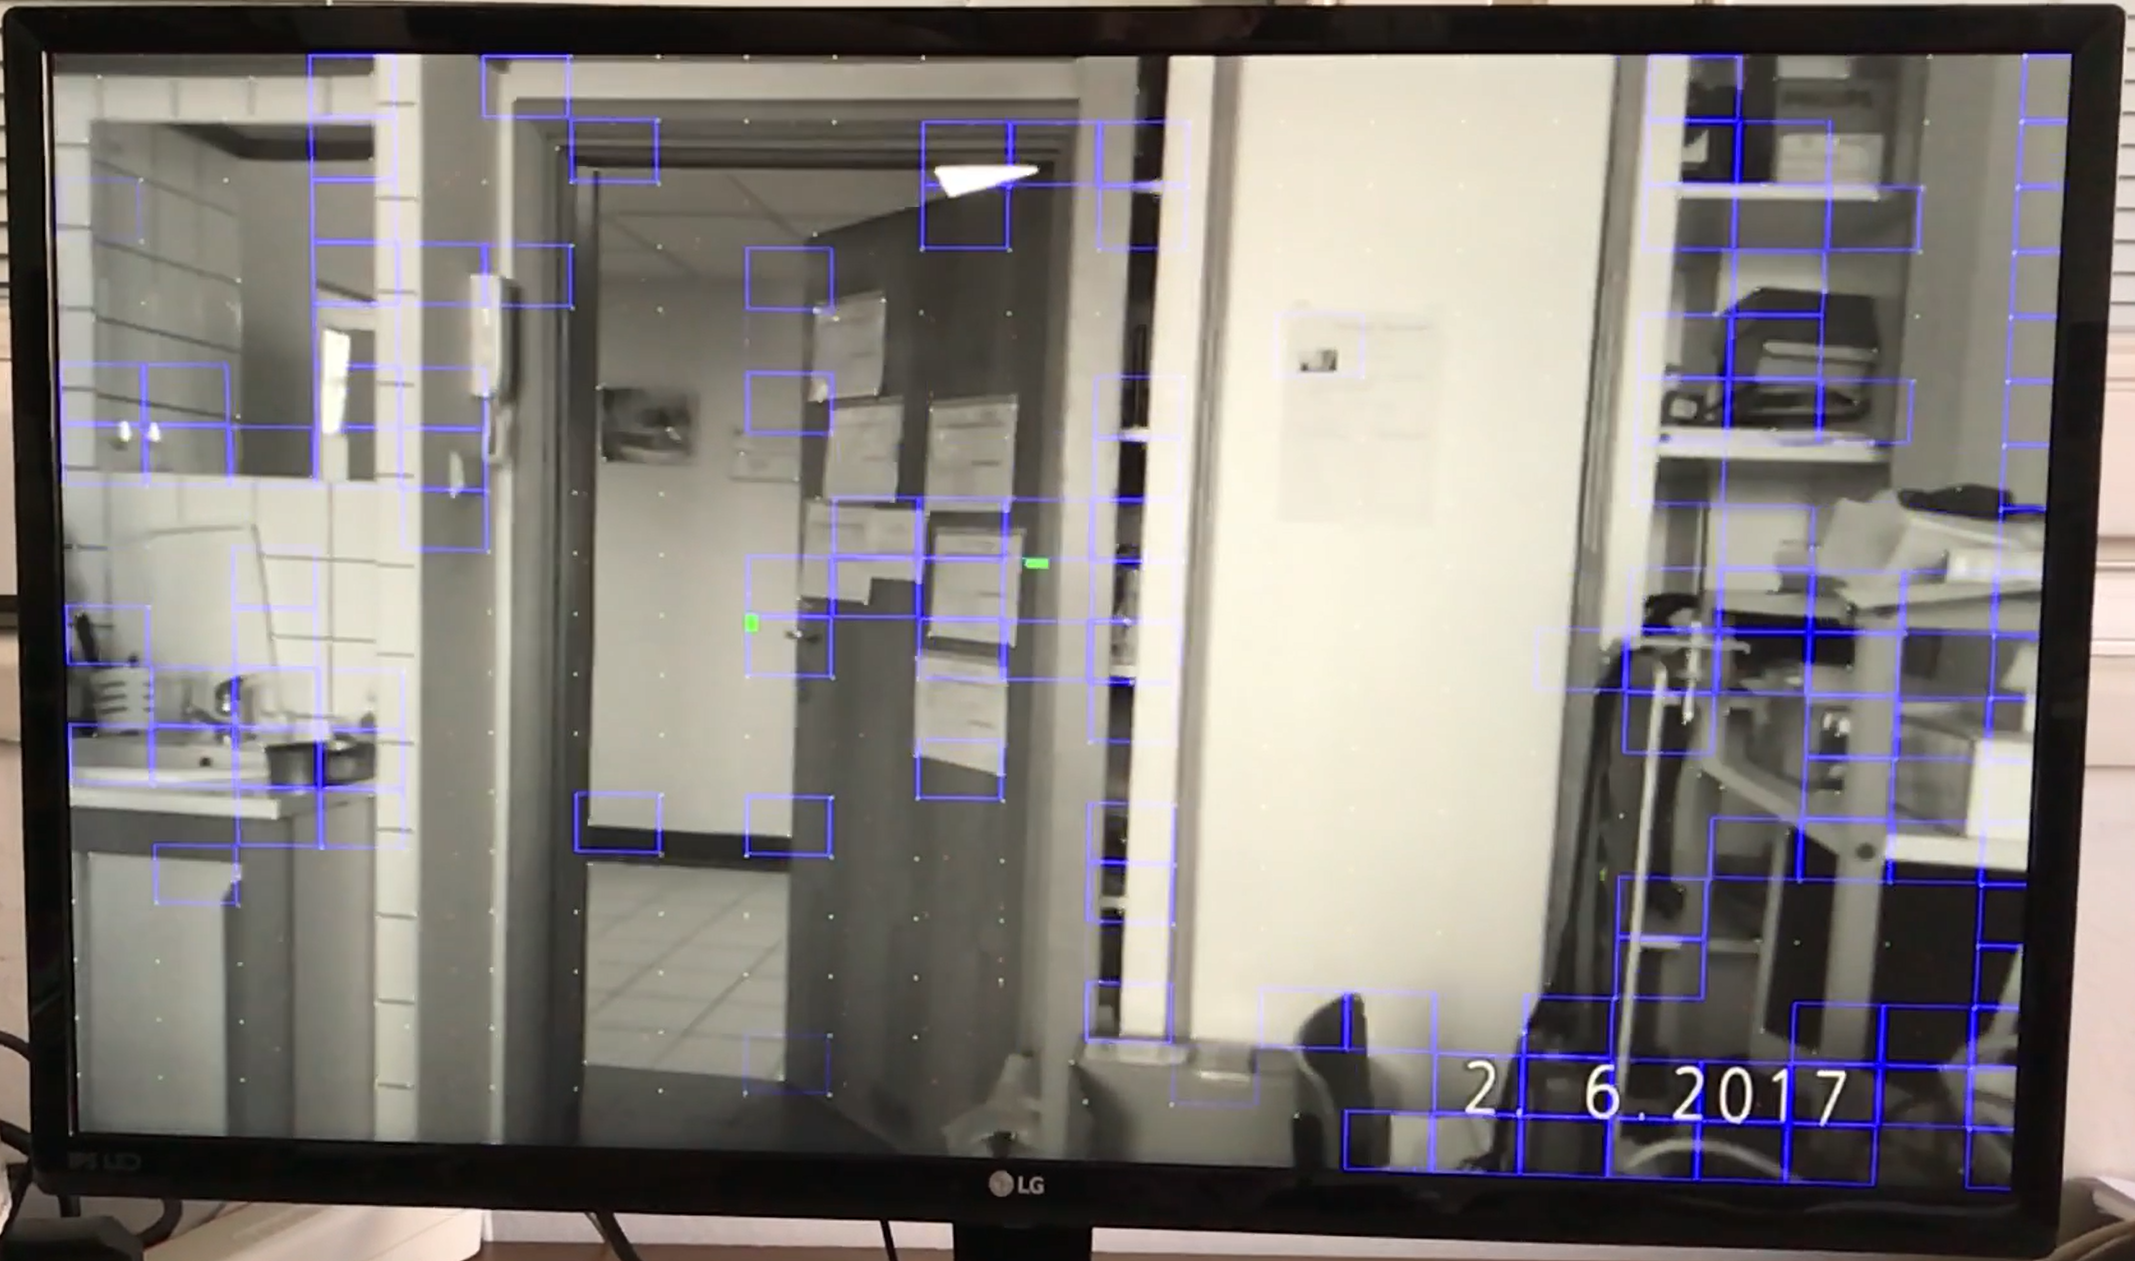
\includegraphics[scale=0.2]{img/4/vibe_plus_example.png}
		\caption{Wizualizacja przepływu optycznego}
		\label{fig:vibe_plus_demo}
	\end{figure}
	

\section{Implementacja algorytmu PBAS}
\label{sec:fpga_pbas}

Szczegółowy opis teoretyczny algorytmu \textit{PBAS} został zamieszczony w podrozdziale \ref{sec:pbas_teoria}. Zaimplementowano wariant operujący w przestrzeni kolorów \textit{RGB} w rozdzielczości \textit{720x576} pikseli oraz wersję przetwarzającą obraz w skali szarości, w przypadku wyższych rozdzielczości (\textit{720p} i \textit{1080p}). Wysokopoziomowy schemat całego algorytmu został przedstawiony na rysunku \ref{fig:pbas_diagram}. Jak zostało już wspomniane w części teoretycznej, wersja algorytmu działająca w przestrzeni \textit{RGB}, przetwarza niezależnie poszczególne składowe, tworząc dla każdej z nich osobny model tła. 
	
	\begin{figure}[h!]
		\centering
		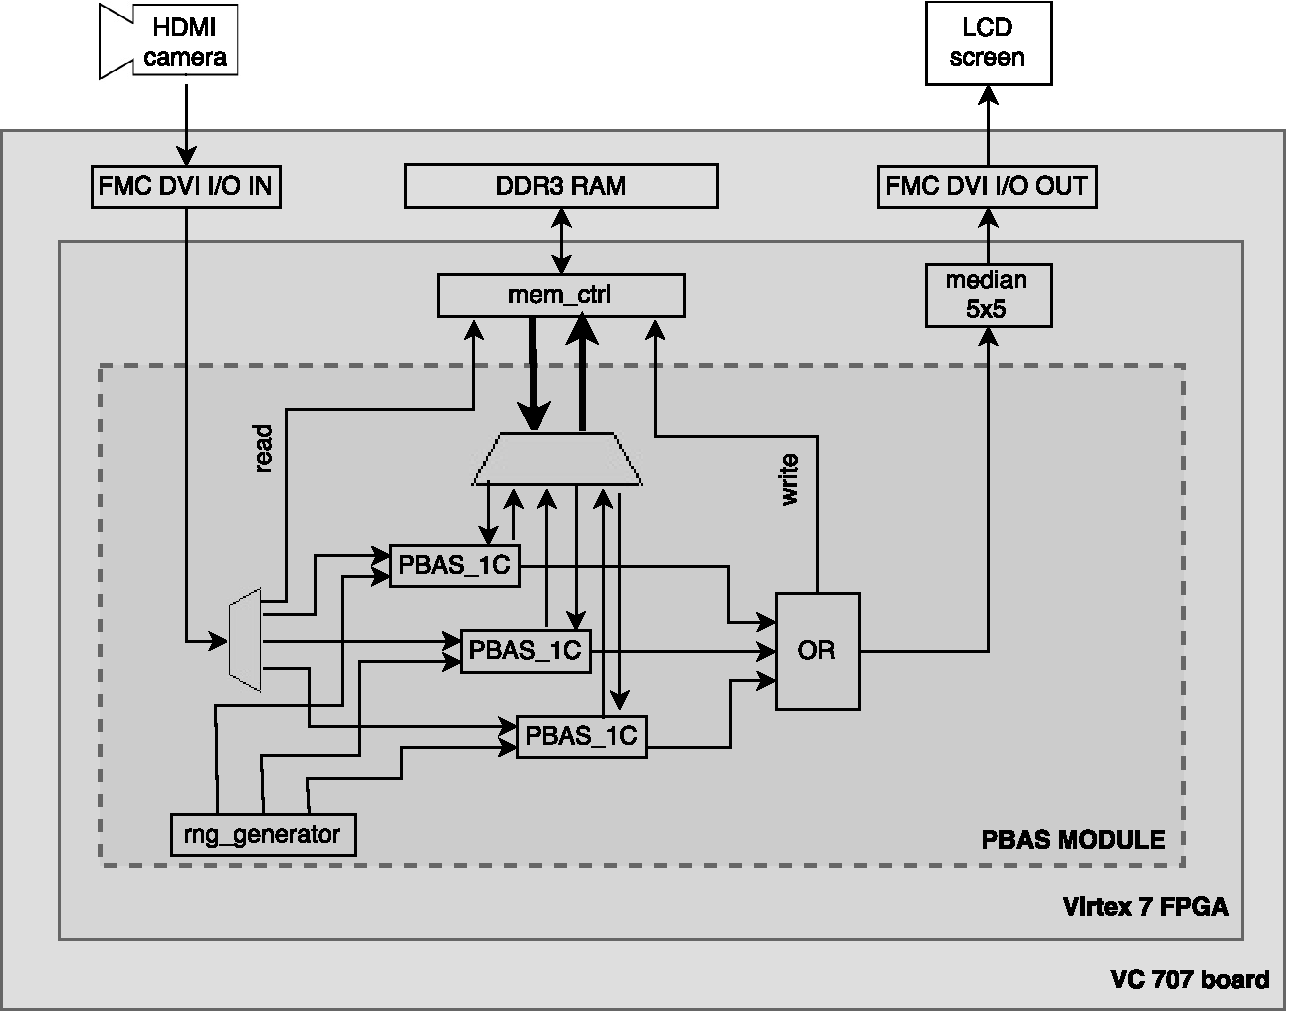
\includegraphics[scale=0.6]{img/4/pbas.pdf}
		\caption{Implementacja algorytmu \textit{PBAS} w wersji \textit{RGB}}
		\label{fig:pbas_diagram}
	\end{figure}

Pierwszą operacją, jest rozbicie sygnału wejściowego na składowe \textit{RGB}. Następnie każda z nich jest analizowana niezależnie poprzez algorytm \textit{PBAS} (blok \textit{PBAS\_1C}). Szczegółowy schemat implementacji modułu, realizującego algorytm dla jednej składowej, przedstawiono na rysunku \ref{fig:pbas_1c_diagram}. Maska finalna stanowi alternatywę logiczną wyników otrzymanych z poszczególnych modułów. Podobnie jak w przypadku innych algorytmów, tutaj także, na koniec, nakładany jest filtr medianowy w celu wyeliminowania szumów i zakłóceń. Algorytm wykorzystuje także generator liczb losowych, zaimplementowany w module \textit{rng\_generator}. Jego opis został szerzej przedstawiony w podrozdziale \ref{subsec:fpga_generator}. Opisywany moduł wykorzystuje oczywiście uniwersalny interfejs wizyjny przedstawiony w rozdziale \ref{sec:uklad_interfejs}. 
	
	\begin{figure}[h!]
		\centering
		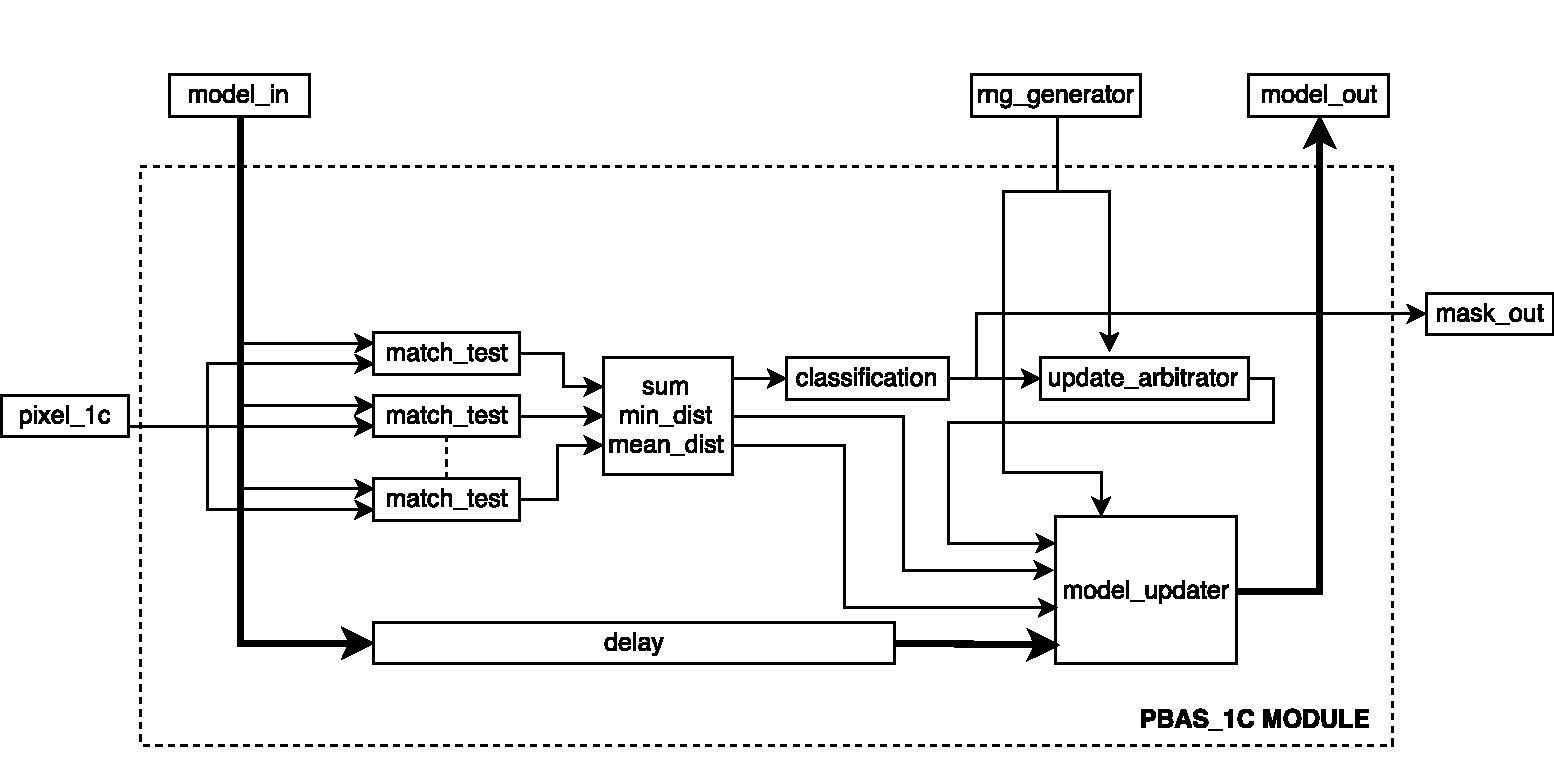
\includegraphics[scale=0.55]{img/4/pbas_1c.pdf}
		\caption{Implementacja algorytmu \textit{PBAS} dla jednej składowej \textit{RGB}}
		\label{fig:pbas_1c_diagram}
	\end{figure}	
	
Implementacja algorytmu \textit{PBAS} przedstawiona na rysunku \ref{fig:pbas_1c_diagram}, operującego na jednej składowej \textit{RGB} bądź skali szarości, jest bardzo podobna do implementacji metody \textit{ViBE} przedstawionej w rozdziale \ref{sec:fpga_vibe}. Podobnie jak w tamtym przypadku, tutaj także, pierwszym krokiem, jest równoległy test dopasowania do próbek zapisanych w pamięci \textit{RAM}, zgodnie z równaniem (\ref{equ:pbas_dist}). Następnie przeprowadzana jest klasyfikacja, opisana równaniem (\ref{equ:pbas_test}). Dodatkowo obliczany jest minimalny dystans pomiędzy próbkami z modelu a aktualnym pikselem oraz średnia wartość odległości zapisanych w modelu tła. Tak samo jak w metodzie \textit{ViBE}, decyzja o podjęciu aktualizacji realizowana jest przez moduł \textit{update\_arbitrator}. Blok dokonujący aktualizacji, jest rozszerzeniem tego co zostało zaprezentowane w implementacji metody \textit{ViBE}. Dodatkowo, oprócz próbek, aktualizowany jest także zbiór minimalnych odległości oraz parametry $R$ i $T$, zgodnie z równaniami (\ref{equ:pbas_r_update}) i (\ref{equ:pbas_t_update}).

Pierwsza część modelu składa się z $N$ próbek, każda próbka zawiera wartość piksela -- $B_i$ oraz zapamiętany minimalny dystans -- $D_i$ pomiędzy aktualną próbką a aktualną wartością piksela. Na końcu znajdują się parametry $R$ i $T$. Modele dla poszczególnych składowych \textit{RGB} ustawione kolejno po sobie. Dla rozdzielczości \textit{576p} przyjęto model składający się z $N=19$ próbek. Parametry $R$ i $T$ zapisano w postaci 16-bitowych liczb stałoprzecinkowych w formacie \textit{8z8u}. Minimalny dystans, podobnie jak próbka, zapisana jest jako 8-bitowa liczba całkowita. Sumarycznie model tła dla jednej składowej \textit{RGB} ma rozmiar $19 \cdot (8+8) + 16 + 16 = 336$ bitów, zatem cały model zajmuje $3 \cdot 336 = 1008$ bitów. Dla wyższych rozdzielczości wykorzystano algorytm operujący na obrazie w skali szarości, model w tym przypadku składa się z $N=14$ próbek. Zatem, cały model, można zapisać za pomocą $14 \cdot (8+8) + 16 + 16 = 256$, jest to maksymalna szerokość modelu, która może zostać wykorzystana w przypadku obrazu w rozdzielczości \textit{720p} lub \textit{1080p}. 


\section{Implementacja rozszerzonej wersji metody PBAS}
\label{sec:fpga_pbas_plus}

Przedstawiona implementacja, powstała na podstawie opisu teoretycznego, zamieszczonego w rozdziale \ref{subsec:pbas_duchy}. Opisana tutaj, rozszerzona wersja algorytmu \textit{PBAS}, zawiera dodatkowy mechanizm rozróżniania obiektów statycznych od tzw. ,,duchów''. Koncepcja ta, wymaga także zaimplementowania metody indeksacji obiektów, co sprawia, że omawiany moduł jest najbardziej złożonym spośród wszystkich pokazanych w niniejszej pracy. Fragmenty przedstawionego tutaj rozwiązania pochodzą z publikacji \cite{kryjak_14_pbas}, również powstałej w Laboratorium Biocybernetyki AGH. Ogólny schemat przedstawiający architekturę modułu pokazano na rysunku \ref{fig:pbas_plus_diagram}. 
	
	\begin{figure}[h!]
		\centering
		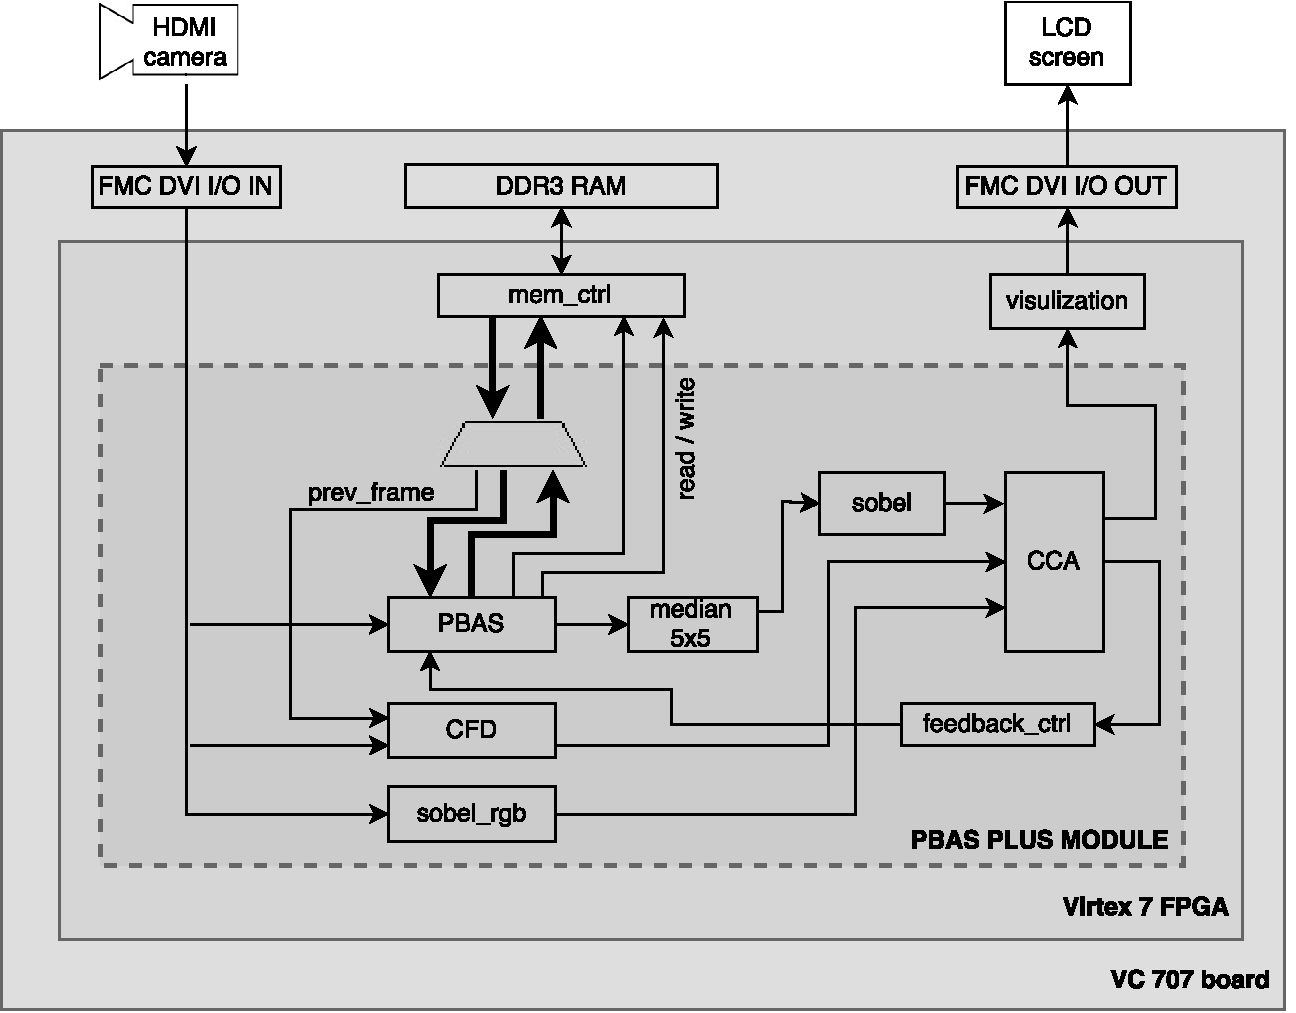
\includegraphics[scale=0.6]{img/4/pbas_plus.pdf}
		\caption{Implementacja rozszerzonej wersji algorytmu \textit{PBAS}}
		\label{fig:pbas_plus_diagram}
	\end{figure}
	
Pierwszym istotnym elementem jest realizacja podstawowego algorytmu \textit{PBAS}, w stosunku do wersji przedstawione w rozdziale \ref{} musiał on zostać zmodyfikowany. Konieczne było dodanie obsługi sprzężenia zwrotnego zgodnie z równaniami (\ref{}) i (\ref{}). Oprócz tego należało także zapewnić aktualizację dwóch nowych parametrów $S(x_i)_{cnt}$ i $E(x_i)_{mean}$, zgodnie z równaniami (\ref{equ:pbas_s_cnt}) i (\ref{equ:pbas_ec_mean}). Dodatkowo w modelu tła musi znaleźć się też poprzednia wartość piksela ($24$ bity) wykorzystywana podczas odejmowania ramek (blok \textit{CFD}). W związku z tym, aby rozmiar modelu nie przekroczył maksymalnego rozmiaru wynoszącego $1024$ bity, konieczne było zredukowanie liczby próbek w algorytmie \textit{PBAS} do $18$. Parametr $S(x_i)_{cnt}$ zapisany jest jako 8 bitowa liczba całkowita, z kolei wartość $E(x_i)_{mean}$ to 16 bitowa liczba stałoprzecinkowa w formacie \textit{8z8u}. Ostatecznie rozmiar modelu tła w takiej konfiguracji wynosi: $3 \cdot (18 \cdot (8+8) + 16 + 16) + 8 + 16 + 24 = 1008$ bitów.

Równolegle do algorytmu \textit{PBAS} wykonywane jest, wspomniane wcześniej, odejmowanie ramek oraz detekcja krawędzi metodą Sobela. Na maskę wyjściową podobnie jak w poprzednich metodach, nakładany jest filtr medianowy. Wyznaczane są także krawędzie na masce binarnej, gdyż jest to niezbędne podczas przeprowadzania analizy poszczególnych obiektów. Schemat bloku \textit{CCA}, odpowiedzialnego za to zadanie, został pokazany na rysunku \ref{fig:cca_diagram}. Ze względu ma fakt, że dane z modułu analizy obiektów dostępne są dopiero po przetworzeniu całej ramki obrazu, konieczne jest zapewnienie odpowiedniej synchronizacji sygnałów sprzężenia zwrotnego z modułem  \textit{PBAS}. Zadanie to zostało zrealizowane poprzez blok \textit{feedback\_ctrl}. Wyznaczone wartości współczynników stabilności i podobieństwa krawędzi oraz finalna maska są zapisywane w pamięci \textit{BRAM}. Działający algorytm, poprawnie identyfikujący obiekt pierwszoplanowy oraz prostokąt go otaczający, został pokazany na rysunku \ref{fig:pbas_plus_demo}.

	\begin{figure}[h!]
		\centering
		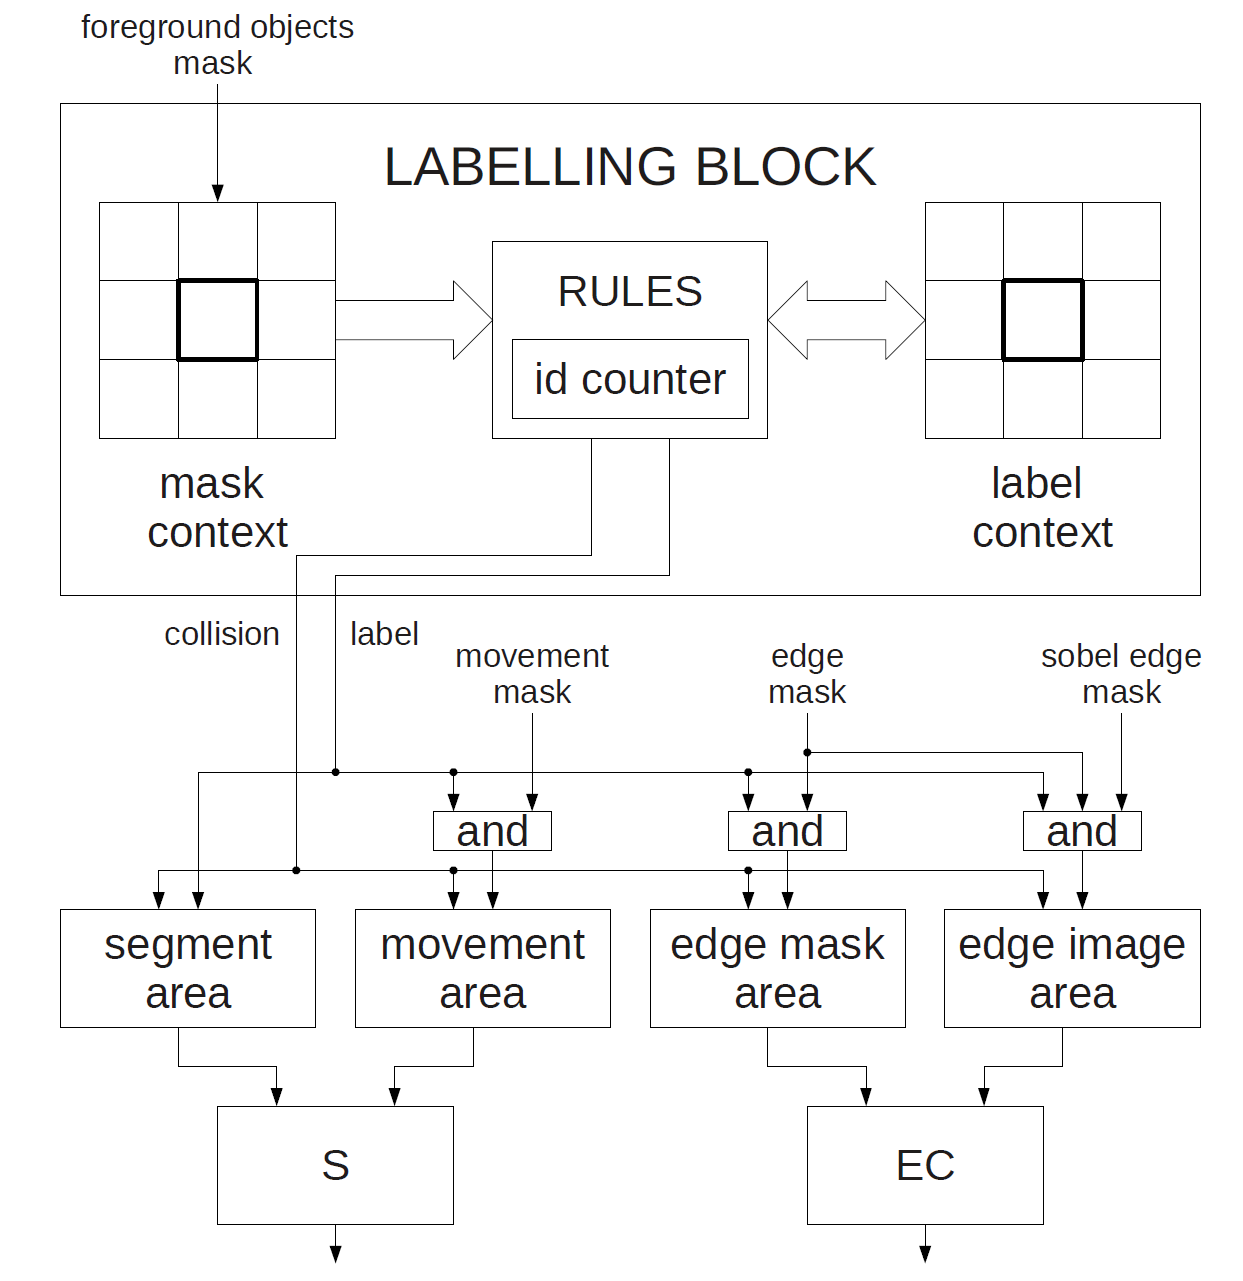
\includegraphics[scale=0.35]{img/4/cca_diagram.png}
		\caption{Architektura modułu \textit{CCA} -- źródło \cite{kryjak_14_pbas}}
		\label{fig:cca_diagram}
	\end{figure}

Do zrealizowania zadania indeksacji obiektów wykorzystano moduł \textit{CCA} opracowany w ramach publikacji \cite{kryjak_14_pbas}. Całość została przygotowana w oparciu o teorię na temat indeksowania obiektów, przedstawioną w rozdziale \ref{subsec:pbas_indeksacja}. Przygotowany moduł składa się z dwóch części, pierwszą z nich jest fragment logiki programowej (\textit{Labelling Block}), odpowiedzialny za przypisanie kolejnym pikselom odpowiednich etykiet. Jak zostało to opisane w części teoretycznej, etykieta jest dobierana na podstawie sąsiednich pikseli oraz etykiet im przypisanych. Konieczne jest zatem wygenerowanie kontekstu piksela wejściowego, zawierającego etykiety przypisane sąsiadom.

Informacja o przydzielonej etykiecie przekazywana jest do czterech bloków obliczających pole zidentyfikowanego obiektu. Pierwszy licznik (\textit{segment area} służy do wyznaczenia całkowitego pola obiektu. Drugi moduł (\textit{movement area}) zlicza natomiast jedynie ruchome piksele. Wartości te są używane do wyznaczenia współczynnika $S_{O_k}$ zgodnie z równaniem \ref{equ:pbas_stability}, wykorzystano w tym celu dzielarkę sprzętową. Kolejny licznik (\textit{edge mask area}) służy do zliczania pikseli na pierwszoplanowej masce krawędzi. Ostatni z modułów (textit{edge image area}) wyznacza liczbę pikseli znajdujących się na wspomnianej wyżej masce oraz na zbinaryzowanym obrazie krawędzi obrazu wejściowego. Te dwie wartości służą do wyznaczenia parametru $EC_{O_k}$, zgodnie z równaniem \ref{equ:pbas_edge_coef}. Podobnie jak w poprzednim przypadku, tutaj także wykorzystano dzielarkę sprzętową.

Oprócz wymienionych czterech istnieje jeszcze jeden blok, aktualizujący na bieżąco parametry prostokąta otaczającego poszczególne obiekty. Wszystkie liczniki zostały zaimplementowane z użyciem pamięci blokowej \textit{BRAM}. Problem konfliktów rozwiązano, poprzez sumowanie wartości zapamiętanych dla obu łączonych obiektów i zapisanie jej jako nowej wartości dla obiektu o niższej etykiecie. Wartość zapisana pod adresem wyższej etykiety zostaje natomiast oznaczona jako nieważna.

	\begin{figure}[h!]
		\centering
		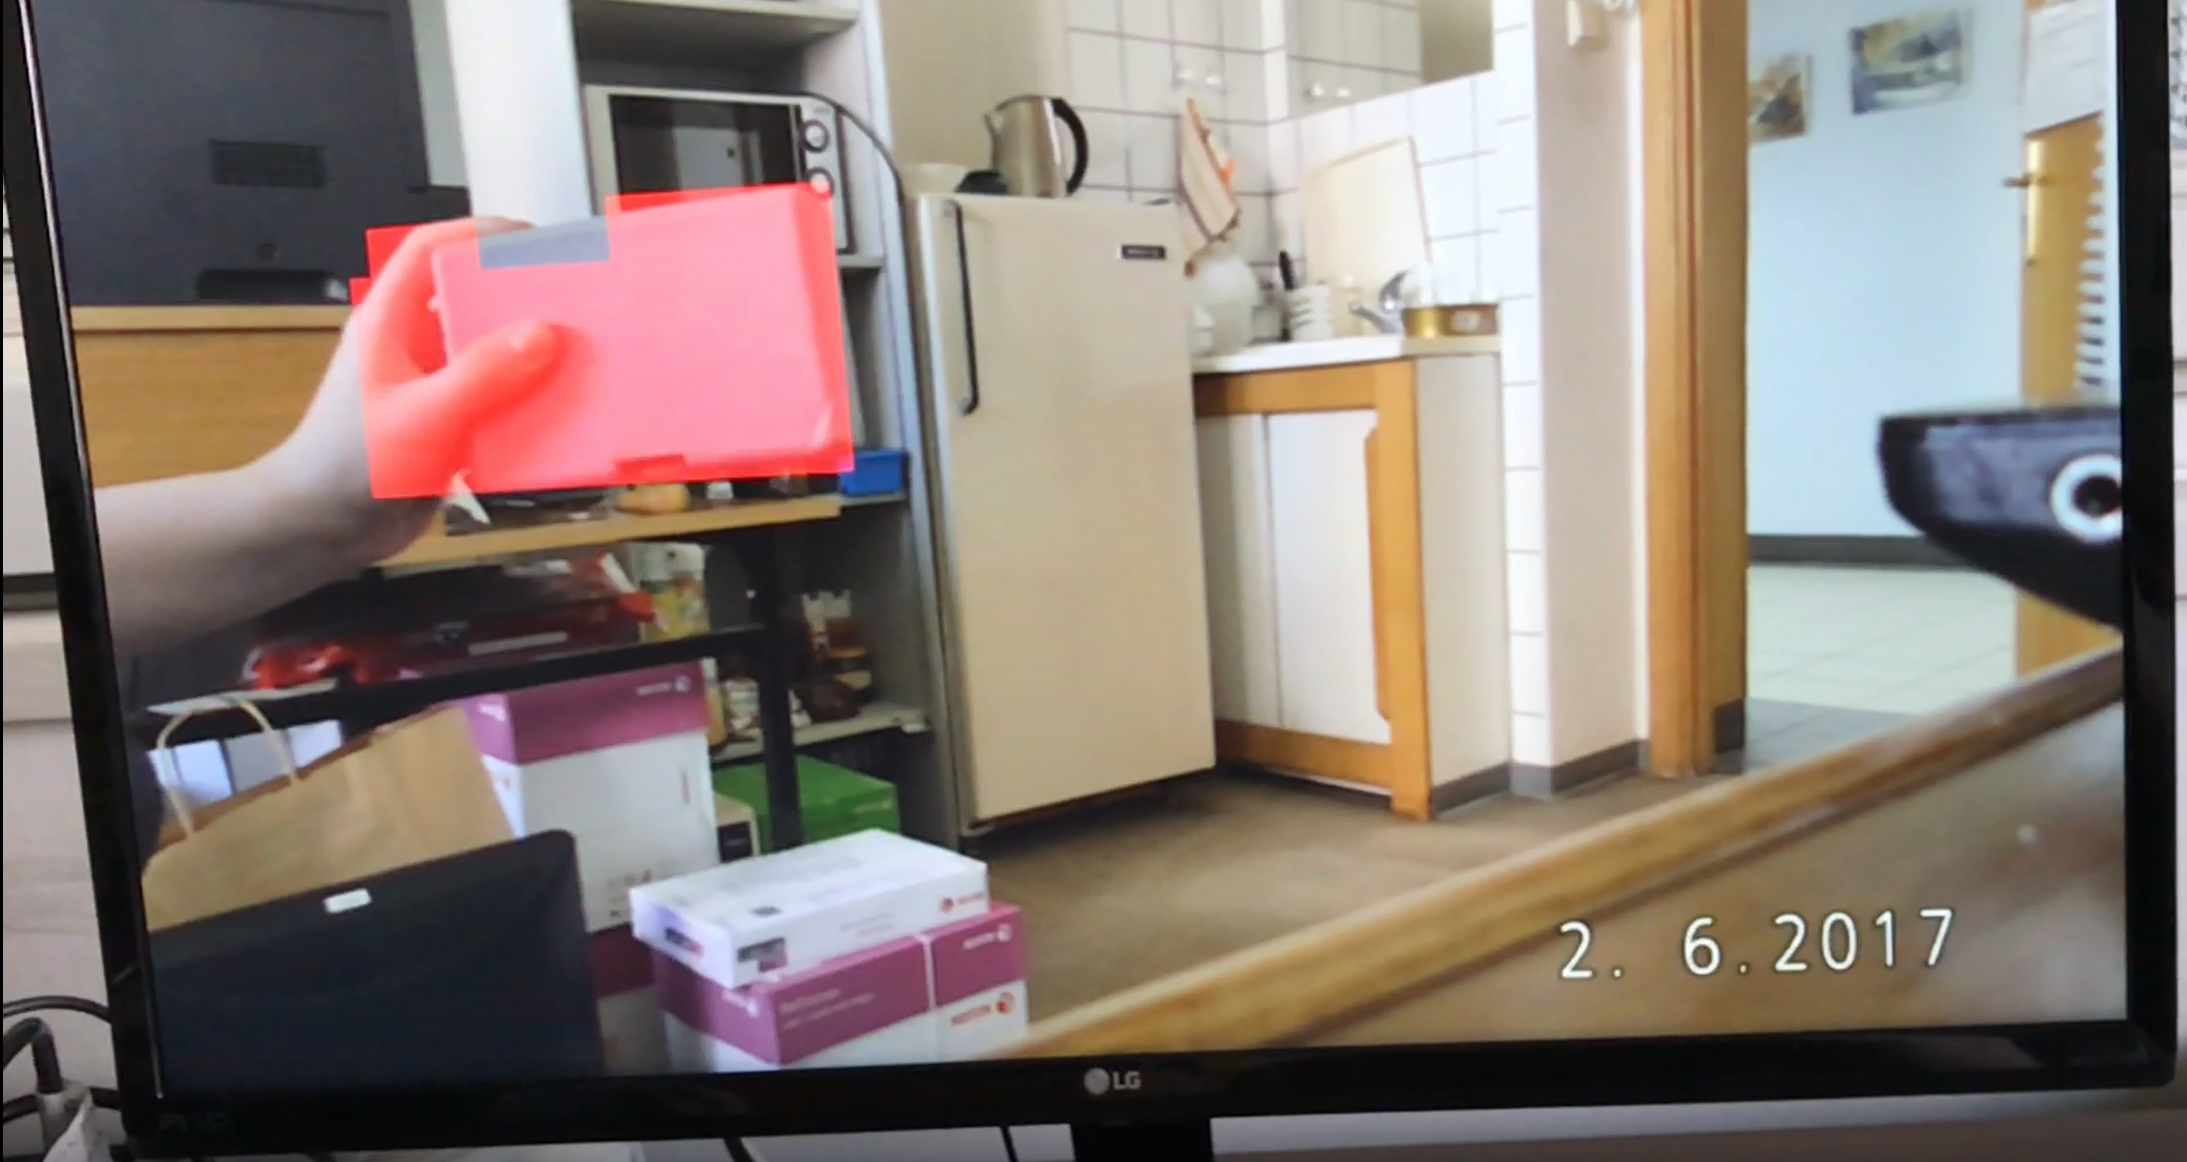
\includegraphics[scale=0.2]{img/4/pbas_plus_example.png}
		\caption{Działający algorytm \textit{PBAS} wraz z indeksacją obiektów}
		\label{fig:pbas_plus_demo}
	\end{figure}

\section{Implementacja GMM}
\label{sec:fpga_gmm}

Przedstawiona tutaj implementacja algorytmu \textit{GMM} została przygotowana w ramach pracy inżynierskiej \cite{piszczek_15}. Sposób implementacji sprzętowej omawianej metody jest tematem niezwykle rozległym, w niniejszym rozdziale przedstawiono jedynie ogólną idee przygotowanej architektury bez zagłębiania się w szczegóły implementacyjne. Schemat przedstawiający implementację i wykorzystane moduły został pokazany na rysunku \ref{fig:gmm_diagram}.

	\begin{figure}[h!]
		\centering
		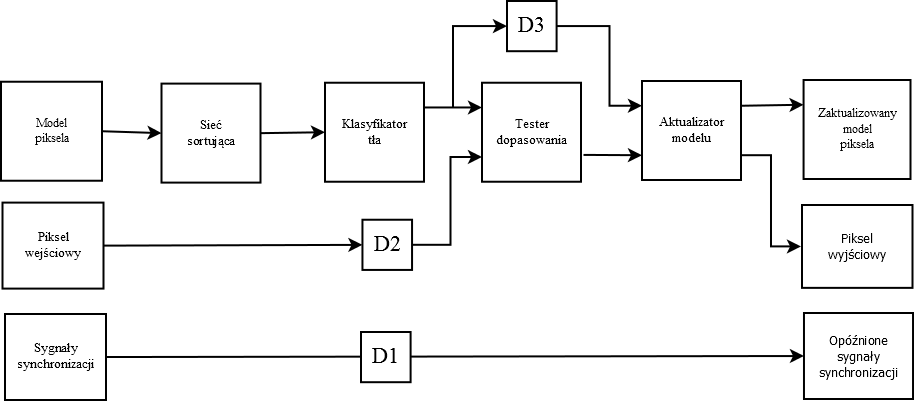
\includegraphics[scale=0.45]{img/4/gmm.png}
		\caption{Implementacja algorytmu \textit{GMM} -- źródło \cite{piszczek_15}}
		\label{fig:gmm_diagram}
	\end{figure}
	
Niewątpliwą zaletą, znacząco ułatwiającą implementację w układzie reprogramowalnym jest brak operacji kontekstowych. Dzięki temu możemy znacząco uprościć logikę programową i zredukować zużycie zasobów. Nawiązując do opisu teoretycznego zamieszczonego w rozdziale \ref{sec:gmm_teoria}, pierwszym krokiem algorytmu jest sortowanie rozkładów Gaussa według współczynnika $r_i = \frac{\omega_i}{\sigma_i}$. W tym celu wykorzystana została specjalnie zaprojektowana sieć sortująca, jest to najbardziej złożony element przedstawianej implementacji. 

Po dokonaniu sortowania, poszczególne rozkłady Gaussa są klasyfikowane, na podstawie równania \ref{equ:gmm_b}. Następnie przeprowadzany jest test dopasowania i ostateczna klasyfikacja piksela, zgodnie z~równaniem \ref{equ:gmm_mahalanobis}. Po dokonaniu klasyfikacji rozkłady Gaussa są aktualizowane i zapisywane w pamięci \textit{RAM}.

Przygotowana implementacja przetwarza obraz we wszystkich wymaganych rozdzielczościach, czyli \textit{576p}, \textit{720p} i \textit{1080p} w 50 klatkach na sekundę. Dla obrazu \textit{720x576} przyjęto $K=5$ rozkładów Gaussa w każdym model, natomiast dla wyższych rozdzielczości, ze względu na ograniczenia pamięci \textit{RAM}, liczba rozkładów wynosi $K=3$. W modelu tła pojedynczy rozkład Gaussa ma rozmiar $68$ bitów, dokładny opis i reprezentacja poszczególnych bitów modelu została przedstawiona w tabeli \ref{tab:gmm_ram_model}.

\begin{table}[h]
	\centering
	\begin{threeparttable}
		\caption{Znaczenie kolejnych bitów w reprezentacji rozkładu Gaussa -- źródło \cite{piszczek_15}}
		\label{tab:gmm_ram_model}

		\begin{tabular}{| c | m{12.5cm} |}  
		\hline
		\textbf{Zakres bitowy} & \multicolumn{1}{c|}{\textbf{Oznaczenie}} \\
		\hline
		\textit{0} & Bit pierwszego planu. Jeśli jest równy 1 oznacza to, że rozkład Gaussa reprezentuje obiekty pierwszoplanowe, w przeciwnym razie reprezentuje on tło. \\
		\hline
		\textit{1 -- 7} & Bity zarezerwowane (w razie wprowadzenia nowych flag). \\
		\hline
        \textit{8 -- 19} & Waga rozkładu Gaussa $\omega$ jako liczba stałoprzecinkowa (zakres 0 -- 1). Część całkowita zajmuje 0 bitów, część ułamkowa 12 bitów. \\
	    \hline
	    \textit{20 -- 31} & Wariancja ($\sigma^2$) jako liczba stałoprzecinkowa (zakres 0 -- 256). Część całkowita zajmuje 8 bitów, część ułamkowa 4 bity. \\
	    \hline
	    \textit{32 -- 43} & Średnia wartość barwy czerwonej piksela jako liczba stałoprzecinkowa (zakres 0 -- 256). Część całkowita zajmuje 8 bitów, część ułamkowa 4 bity. \\
        \hline
        \textit{44 -- 55} & Średnia wartość barwy zielonej piksela jako liczba stałoprzecinkowa (zakres 0 -- 256). Część całkowita zajmuje 8 bitów, część ułamkowa 4 bity. \\
        \hline
        \textit{56 -- 67} & Średnia wartość barwy niebieskiej piksela jako liczba stałoprzecinkowa (zakres 0 -- 256). Część całkowita zajmuje 8 bitów, część ułamkowa 4 bity. \\
        \hline
		\end{tabular}				
	\end{threeparttable}
\end{table}

Poglądowy schemat przedstawiający zasadę działania sieci sortującej dla $K=5$ elementów, został pokazany na rysunku \ref{fig:gmm_sort}. Jest to sprzętowa realizacja algorytmu \textit{BS} (ang. \textit{Bubble Sort} -- sortowanie bąbelkowe). Pionowe linie oznaczają, porównania między elementami. Przerywane linie z grotem określają z kolei kierunek przesuwania się najmniejszego elementu w danej iteracji. W pierwszym kroku spośród $K$ elementów, wyłaniany jest najmniejszy poprzez wykonanie $K-1$ porównań. Wyznaczony w ten sposób element jest przestawiany na sam dół sieci. Następnie wśród pozostałych $K-1$ elementów wyszukiwany jest kolejny najmniejszy, w tym przypadku należy wykonać $K-2$ porównania itd. Ostatecznie do otrzymania posortowanego ciągu potrzeba $K-1$ iteracji algorytmu.  
	
	\begin{figure}[h!]
		\centering
		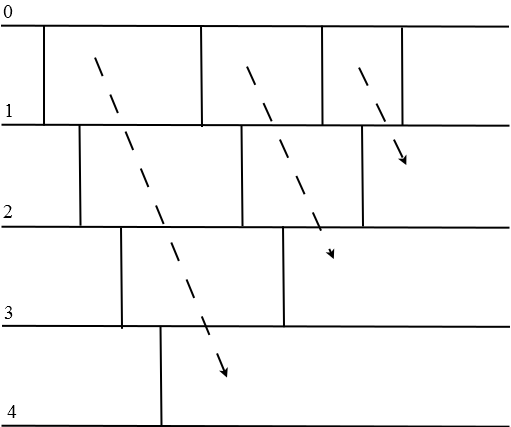
\includegraphics[scale=0.4]{img/4/sort_module.png}
		\caption{Sieć sortująca w układzie \textit{FPGA} -- źródło \cite{piszczek_15}}
		\label{fig:gmm_sort}
	\end{figure}	


\section{Zużycie zasobów}
\label{sec:fpga_zasoby}